
%\documentclass[oribibl]{llncs}
\documentclass{report}

\usepackage{times}
\usepackage{stmaryrd, latexsym, amsmath, amssymb, wasysym}
\usepackage{fancyvrb}

\usepackage{semantic}

\usepackage{epic,eepic}
\usepackage{graphicx}
\usepackage{caption}
\usepackage{array}

% Time-stamp: <2006-08-24 16:37:12 Andrei Sabelfeld> 


\newcommand{\prefix}[2]{\ensuremath{\mathit{prefix}(#1,#2)}}
\newcommand{\foreverhigh}{\ensuremath{\Rightarrow_\high}}


\newcommand{\RuleSideCond}[4]
{\centerline{
   { \ensuremath{
           \mprset{flushleft}
           \inferrule*[Left=#1, Right=#4]
           {#2}
           {#3}
         }
   }
}}

\newcommand{\spp}{\hspace{2pt}} 
\newcommand{\hh}{\ensuremath{\hbar}}
\newcommand{\islow}{\ensuremath{low?}}


%%%%%%%%%%%%%%%%%%%%%%%%                  some macros             %%%%%%%%%%%%%%%%%%%%%%%%%%%%

% Proofs

% For proofs% PROOF ENVIRONMENT (from PT)
% it puts a box (or whatever \markendofproof) at the end of each
% proof, unless the author has already done so with the command \qed.
 
% the ``proof'' environment itself

% \newcommand{\scfont}[1]{{\sc #1}} % renew this for latex2e
\def\proof{\followon{Proof}}
\def\endproof{\ifSuppressEndOfProof\global\SuppressEndOfProoffalse
   \else\xqed\fi\endfollowon}
\def\followon#1{\trivlist\item[\hskip\labelsep{\textbf{#1}.}]}
\def\endfollowon{\endtrivlist}

% command to push box to right of page
\def\pushright#1{{\parfillskip=0pt\widowpenalty=10000
\displaywidowpenalty=10000\finalhyphendemerits=0\leavevmode\unskip
\nobreak\hfil\penalty50\hskip.2em\null\hfill{#1}\par}}

% command to force early end of proof marker. This is used if the end
% of proof marker would otherwise come out in the wrong place.
\def\qed{\xqed\global\SuppressEndOfProoftrue}
\newif\ifSuppressEndOfProof\SuppressEndOfProoffalse
\def\xqed{\pushright\markendofproof}
\def\markendofproof{$\Box$} % rule{1.3217ex}{2ex}}


%\newcommand{\proofbeg}{\par{\bf Proof. }}
%\newcommand{\proofsketch}{\par{\bf Proof sketch. }}
%\newcommand{\proofend}{\mbox{$\Box$}}

\newcommand{\corol}{\par{\bf Corollary. }}

\newcommand{\ex}{\par{\bf Example. }}

\newcommand{\draft}{{\bf \fbox{DRAFT}}}

\newtheorem{Theorem}{Theorem}
\newtheorem{Proposition}{Proposition}
\newtheorem{Corollary}{Corollary}
\newtheorem{Lemma}{Lemma}
\newtheorem{Definition}{Definition}
\newtheorem{Observation}{Observation}

\newcommand{\nb}[1]{$\blacktriangleleft$\ {\bf #1\/} $\blacktriangleright$\ 
\marginpar{{\bf NB}}}                     % for visible comments;
%\newcommand{\nb}[1]{}                   % select this line to hide them

\newcommand{\nat}{\mathbb{N}} 
%\newcommand{\nat}{{\boldmath N}} 
%\newcommand{\equals}{\stackrel{.}{=}}

%\newcommand{\para}[2][]{\prod_{#1} #2} 
%\newcommand{\para}[2][]{\! <\! #2\! >_{#1}\!} 
\newcommand{\para}[1]{\langle #1 \rangle}
\newcommand{\paral}{\mid}

% experiments to tame the latex8 sf

%\renewcommand{\sfdefault}{phv,10pt}

%  add the period after section numbers 

%\renewcommand{\section}[1]{\Section{\hskip -1em.~#1}} 
%\renewcommand{\subsection}[1]{\SubSection{\hskip -1em.~#1}}
                                       
%% a hack for latex8 style

%\newfont{\emailfont}{phv12}

\newcommand{\codcaption}[1]{\mathtt{#1}}
%\newcommand{\codemail}[1]{\textsf{\normalsize #1}}
%\newcommand{\codfoot}[1]{{\fontfamily{phv}\fontsize{7}{.3cm}\selectfont #1}}
%\newcommand{\codsubsec}[1]{\textsf{\normalsize #1}}

% from former dec-dave.tex

\newcommand{\cod}[1]{\mathtt{#1}} % program text   
                                          %% \small was 
                                          %% a hack for latex8 style
\newcommand{\true}{\cod{True}}
\newcommand{\false}{\cod{False}}
\newcommand{\If}{\cod{if}}
\newcommand{\ifthenelse}[3]{\cod{if}~#1~\cod{then}~#2~\cod{else}~#3}
\newcommand{\ifthen}[2]{\cod{if}~#1~\cod{then}~#2}
\newcommand{\while}[2]{\cod{while}~#1~\cod{do}~#2}
\newcommand{\Int}{\mathit{Int}} % Type of Integers
\newcommand{\choice}{\talloblong}
\newcommand{\await}[2]{\cod{await}~#1~\cod{then}~#2}
\newcommand{\spawn}[1]{\cod{spawn}~#1}
\newcommand{\fork}[2]{\cod{fork}(#1,#2)}
\newcommand{\forkproc}[2]{\ensuremath{\lambda}#1.#2}
\newcommand{\forklocalvars}[3]{\cod{fork}((\forkproc{#1}{#2})\, @ \, #3)}

\newcommand{\out}[1]{\cod{output}(#1)}

\newcommand{\hforkbyvalue}[3]{\cod{hfork}_{[#1]}(#2,#3)}

\newcommand{\hide}{\cod{hide}}
\newcommand{\edih}{\cod{unhide}}
\newcommand{\yield}{\cod{yield}}
\newcommand{\hfork}[2]{\cod{hfork}(#1,#2)}
\newcommand{\Loop}{\cod{loop}}
\newcommand{\Skip}{\cod{skip}}
\newcommand{\Empty}{\emptyset}
\DeclareMathAccent{\arrowvec}{\mathord}{letters}{"7E}
\newcommand{\vect}[1]{\arrowvec{#1}}              % LaTeX 2.09 
\newcommand{\const}[1]{\mbox{\it #1}}
%\newcommand{\halt}{\cod{stop}}
\newcommand{\halt}{\mathit{stop}}
%\renewcommand{\vec}[1]{\error}   

\newcommand{\decl}[1]{\cod{declassify}(#1)}


% Synchronisation
\newcommand{\wait}[1]{\cod{P}(#1)}
\newcommand{\signal}[1]{\cod{V}(#1)}
\newcommand{\sem}{\mathit{s}}
\newcommand{\Sem}{\mathit{Sem}}
\newcommand{\newSem}[1]{\cod{newSem}(#1)}
\newcommand{\gSem}{\mathit{w}}   % Global semaphore in a thread
\newcommand{\nSem}{\mathit{s}}   % Global semaphore in a thread
\newcommand{\bSem}{\mathit{b}}   % Global semaphore in a thread

\newcommand{\va}[1]{\mathit{#1}} % to be used for variables
\newcommand{\comment}[1]{\cod{/*}\ \text{#1}\ \cod{*/}}


%\newcommand{\blocked}[2]{\cod{blocked}(#1,#2)}
%\newcommand{\signalled}[2]{\cod{signalled}(#1,#2)}
%\newcommand{\labblocked}{\mathit{blocked}}
%\newcommand{\labsignalled}{\mathit{signalled}}
\newcommand{\labblocked}[1]{\otimes#1}
\newcommand{\labsignalled}[1]{\odot#1}

\newcommand{\syncConfig}[3]{\llocal #1,#2,#3 \rlocal}

\newcommand{\Config}[4]{\llocal \para{#1},#2,#3,#4 \rlocal}

% Semantics

%\newcommand{\union}{\mathord{\cup}}
\newcommand{\Mod}{\mathbin{\mathbf{mod}}}

\newcommand{\term}{\downarrow}

\newcommand{\configs}{\mathit{Config}}
\newcommand{\commands}{\mathit{Com}}
\newcommand{\pools}{\vect{\commands}}


\newcommand{\config}[2]{\langle #1,#2 \rangle}

\newcommand{\llocal}{\langle\hspace{-2.4 pt}|}
\newcommand{\rlocal}{|\hspace{-2.4 pt}\rangle}
%\newcommand{\config}[3]{\langle #1,#2,#3 \rangle}
%\newcommand{\configF}[2]{\langle #1,#2 \rangle}
\newcommand{\configF}[1]{\langle \halt,#1 \rangle}

\newcommand{\configE}[3]{\langle #1,#2,#3 \rangle}
\newcommand{\configEF}[2]{\langle #1,#2 \rangle}

\newcommand{\emptyConfig}{\para{}}
\newcommand{\emptyVec}{\para{}}

\newcommand{\detarrow}{\rightarrowtriangle}
%\newcommand{\labarrow}[1]{\stackrel{#1}{\longrightarrow}}
%\newcommand{\labarrow}[1]{\stackrel{#1}{\rightarrowtriangle}}
\newcommand{\probarrow}[1]{\rightarrow_{#1}}
\newcommand{\parrow}{\rightarrow}
\newcommand{\concarrow}{\rightarrow}

\newcommand{\psetarrow}[1]{\probarrow{#1}}     % the same as \probarrow for the moment

\newcommand{\thread}[1]{\ensuremath{c_{#1}}}
\newcommand{\threadp}[1]{\ensuremath{c'_{#1}}}

\newcommand{\nthreads}
{
 \thread{1}
 \dots
 \thread{n}
}

\newcommand{\selectthread}[4]
{
 \thread{1}
 \dots
 {#1}
 {#2}
 {#4}
 {#3}
 \dots
 \thread{n}
}


\newcommand{\nthreadsp}
{
 \threadp{1}{f_1}
 \dots
 \threadp{n}{f_n}
}

\newcommand{\create}{\leadsto}
\newcommand{\createClose}{\leadsto^*}

\newcommand{\newthreads}{{\vect{d}}} 
\newcommand{\namethreads}[1]{N(#1)}


\newcommand{\cnt}{\textrm{cnt}} % count field of semaphore
\newcommand{\que}{\textrm{que}} %  queue field of semaphore

% Memory / Lock Sets

\newcommand{\mem}{m}
\newcommand{\lockset}{\omega}
\newcommand{\hiddenthreads}{\phi}

% Schedulers semantic

\newcommand{\Schdlconfig}[2]
{\llocal #1, #2 \rlocal}

\newcommand{\Schdlresult}[2]
{\llocal #1, #2 \rlocal}

\newcommand{\hidearrow}[1]{\labarrow{#1 \leadsto \bullet}}
\newcommand{\ediharrow}[1]{\labarrow{\bullet \leadsto #1}}
\newcommand{\yieldarrow}{\labarrow{\leadsto \!\!\!\!/}}
\newcommand{\hiddenforkarrow}{\labarrow{\bullet}}
\newcommand{\hiddenforkarrowvect}[1]{\labarrow{\bullet_{\vect{#1}}}}
\newcommand{\hiddenforkarrowvectbyvalue}[2]{\labarrow{\bullet_{\vect{#1}}\ ,\  #2}}
\newcommand{\forkarrow}{\labarrow{\circ}}
\newcommand{\forkarrowvect}[1]{\labarrow{\circ_{\vect{#1}}}}
\newcommand{\nonfinishedstep}[1]{\labarrow{#1 \, \leadsto}} 
\newcommand{\finishedstep}[1]{\labarrow{#1 \, \leadsto \times}} 
\newcommand{\pickupthread}[1]{\labarrow{\uparrow {#1}}} 
\newcommand{\pickuphighthread}[1]{\labarrow{\uparrow_s{#1}}} 
\newcommand{\choosescheduler}[2]{\labarrow{\otimes{#1}{#2}}} 
\newcommand{\lockedthread}[2]{\labarrow{\labblocked{#1}_{#2}}} 
\newcommand{\signaledthread}[2]{\labarrow{\labsignalled{#1}_{#2}}}

\newcommand{\multiconfig}[4]
{ 
  {\llocal #1,#2,#3,#4 \rlocal}
}

% Schedulers

%\newcommand{\hist}{\Xi}  % too squiggly
\newcommand{\hist}{Hist}
\newcommand{\emptyHist}{\epsilon}
\newcommand{\live}[1]{live(#1)}

\newcommand{\schedule}{\sigma}
\newcommand{\scheduleMem}{\eta}

% Types etc

\newcommand{\high}{\mathit{H}}
\newcommand{\low}{\mathit{L}}
\newcommand{\cmd}[1]{\mathit{#1\ cmd}}
\newcommand{\var}[1]{\mathit{#1\ var}}
\newcommand{\To}{\rightarrow} % function space / type arrow

% Bisimulations

\newcommand{\peq}{\sim_L}
\newcommand{\pseq}[1]{\sim_L^{#1}}
\newcommand{\psieq}{\approx_L}
\newcommand{\pstrong}{\approxeq_L}

\newcommand{\possim}{\preceq}
\newcommand{\posbisim}{\simeq}



% Distribution

\newcommand{\distr}[1]{{\cal D}(#1)}

% --- PERS etc-----------------------
%\newcommand{\Rel}[1]{\mathit{Rel}(#1)} % Relations on A 
\newcommand{\Per}[1]{\mathit{Per}(#1)} % Pers on A
\newcommand{\Domain}[1]{\mathit{dom}(#1)}          % The domain of a relation
\newcommand{\Ker}[1]{\mathit{ker}(#1)} % The kernal of a function
\newcommand{\All}{\mathit{All}}
\newcommand{\Id}{\mathit{Id}}
\newcommand{\Permap}{\rightarrowtriangle} % the per arrow (exponent)

% Domains etc 
\newcommand{\State}{\mathbf{St}}


% Logical ops (for use in Math mode)
\newcommand{\Implies}{\Longrightarrow}
\newcommand{\isimpliedby}{\Leftarrow}
\newcommand{\Iff}{\Longleftrightarrow}


% iff is predefined % \newcommand{\iff}{\Leftrightarrow}

\newcommand{\isbydef}{\stackrel{\mbox{\tiny def}}{=}}
\newcommand{\AND}{\mathrel{\wedge}}
\newcommand{\OR}{\mathrel{\vee}}
% \newcommand{\Subset}{\subseteq}
\newcommand{\Powerset}{\wp}
\newcommand{\Set}[1] % gives a set containing its arg.
           {\left\{#1\right\}}


\newcommand{\lmulti}{\{\hspace{-2.5 pt}|}
\newcommand{\rmulti}{|\hspace{-2.5 pt}\}}
\newcommand{\multiset}[1] % gives a set containing its arg.
           {\lmulti#1\rmulti}

\newcommand{\Setminus}{\setminus}
\newcommand{\SetDef}[2] % {x}{y} => { x | y }
           {\left\{#1\mathrel{\mid}#2\right\}}
\newcommand{\Union} {\cup}
\newcommand{\Intersect} {\cap}
\newcommand{\ForAll}[2]
           {\forall #1 .\,#2}
\newcommand{\Exists}[2]
           {\exists #1 .\,#2}
\newcommand{\entails}{\vdash}
%\newcommand{\Nat}{I\!\!N}

% SIMPLE INFERENCE RULES

% added an optional parameter (a side condition)
\newcommand{\Infer}[3] %  name X top X bottom, ie
                       %    #2
                       % #1---- 
                       %    #3
{\displaystyle \mbox{\footnotesize{#1}}
               \frac{\displaystyle{#2\vspace{.4cm}}}
                    {#3}
} 

% added an optional parameter (a side condition) for use in xalign
\newcommand{\Inferr}[3] %  name X top X bottom, ie
                       %        #2
                       % (#1)   ---- 
                       %        #3
{[#1]&&\displaystyle &\frac{\displaystyle{#2\vspace{.4cm}}}
                                         {#3}
}

\newcommand{\InferrA}[3] %  name X top X bottom, ie
                       %        #2
                       % (#1)   ---- 
                       %        #3
{[#1]\displaystyle &\frac{\displaystyle{#2\vspace{.4cm}}}
                                         {#3}
}

% added an optional parameter (a side condition) for use in xalign
% \newcommand{\Rule}[2]  %  name X top X bottom, ie
%                        %          
%                        % (#1)   #2
%                        %          
% {[#1]&&\displaystyle &\displaystyle{#2}
% }

% \newcommand{\RuleA}[2]  %  name X top X bottom, ie
%                        %          
%                        % (#1)   #2
%                        %          
% {[#1]&\displaystyle{#2}
% }

% Transformation to avoid timing leaks

\newcommand{\transto}{\hookrightarrow}
\newcommand{\transtohigh}{\hightransto}

% Misc

\newcommand{\eol}{\\[.8em]}
\newcommand{\Eol}{\\[1.5em]}

\newcommand{\sS}{{\scriptstyle\mathbb{S}}} % state of Skou's pbisimulation
\newcommand{\tT}{{\scriptstyle\mathbb{S}}'} % state of Skou's pbisimulation

%\newcommand{\sS}{s\hspace{-3.7 pt}s} % state of Skou's pbisimulation

% Formatting

%Compact headings
% \newcommand{\Subsection}[1]{\paragraph{\rm\textbf{#1.}}}
% \newcommand{\Paragraph}[1]{\textbf{#1}}
% \newcommand{\Term}[1]{\textbf{#1}}

%Full headings
%\newcommand{\Subsection}[1]{\subsection{#1}}
%\newcommand{\Paragraph}[1]{\paragraph{#1}}

\newcommand{\cfg}{\mathit{cfg}}
\newcommand{\cfgm}{\mathit{cfgm}}
\newcommand{\configTop}[3]{\langle   #2 ~ |_{#1} ~ #3  \rangle}

\newcommand{\stutterarrow}{\parrow^{\star}}

%%%%%%%%%%%%%%%%%%%%%%%%%%%%%%%%%%%%%%%%%%%%%%%%%%%%%%%%%%%%%%%%%%%%%
%Dec 2005
%%%%%%%%%%%%%%%%%%%%%%%%%%%%%%%%%%%%%%%%%%%%%%%%%%%%%%%%%%%%%%%%%%%%%

\newcommand{\G}{\Gamma}
\newcommand{\proves}{\ensuremath{\vdash}}

\newcommand{\barrier}{\mathit{barrier}}
\newcommand{\semP}[1]{\cod{p}(#1)}
\newcommand{\semV}[1]{\cod{v}(#1)}
%\newcommand{\lock}{\semP{\mathit{lock}}}
%\newcommand{\unlock}{\semV{\mathit{lock}}}
\newcommand{\lock}{\cod{lock}}
\newcommand{\unlock}{\cod{unlock}}
\newcommand{\hightransto}{\looparrowright}

\newcommand{\Rule}[2]{\infer{#2}{#1}} % this uses the proof package
\newcommand{\labRule}[3]{\infer[#1]{#3}{#2}} % this uses the proof package

\newcommand{\Vars}[1]{\mathit{Vars}(#1)}
\newcommand{\IDs}{\mathit{IDs}}
\newcommand{\Vals}{\mathit{Vals}}

\newcommand{\Rel}{\mathit{Rel}}

\newcommand{\configTwo}[2]{\langle #1,#2 \rangle}
\newcommand{\configThree}[3]{\langle #1,#2,#3 \rangle}

%\newcommand{\down}{\mathit{D}}
%\newcommand{\up}{\mathit{U}}

\newcommand{\vars}{\mathit{Vars}}

\newcommand{\inter}{\ensuremath{\cap}}
\newcommand{\union}{\ensuremath{\cup}}

\newcommand{\pc}{\mathit{pc}}
\newcommand{\join}{\sqcup}


%%%%%%%%%%%%%%%%%%%%%%%%%%%%%%%%%%%%%%%%%%%%%%%%%%%%%%%%%%%%%%%%%%%%%
%Dec 2005 - Ale
%%%%%%%%%%%%%%%%%%%%%%%%%%%%%%%%%%%%%%%%%%%%%%%%%%%%%%%%%%%%%%%%%%%%%
\if 0
\newcommand{\mat}[1]{\ensuremath{#1}}
\newcommand{\word}[1]{\textsl{#1}}
\newcommand{\Assgn}{\ensuremath{\Gamma}}
\newcommand{\AssgnOk}{\ensuremath{\Gamma_{\nu}}}
\newcommand{\ofType}[3]{\ensuremath{#1 \vdash #2 : #3}}
\newcommand{\FV}[1]{\word{FV}\mat{(#1)}}
\newcommand{\pc}{\word{pc}}
\newcommand{\hc}{\word{hc}}
\newcommand{\join}{\mat{\sqcup}}

\newcommand{\ND}{\mathit{ND}}
\newcommand{\RR}{\mathit{RR}}
\newcommand{\ws}{\mathit{ws}}
\fi

\newcommand{\monstack}{\mathit{st}}
%\newcommand{\configM}[2]{\langle #1,#2 \rangle}
\newcommand{\configM}[1]{#1}
\newcommand{\larrow}[1]{\stackrel{#1}{\longrightarrow}}
\newcommand{\nop}{\mathit{nop}}
\newcommand{\levelof}[1]{\mathit{lev}(#1)}
\newcommand{\labarrow}[2]{{\stackrel{#1}{\longrightarrow}}_{#2}}
\newcommand{\nolabarrow}{\longrightarrow}
\newcommand{\monitorevent}{\alpha}
\newcommand{\cend}{\mathit{end}}

\newcommand{\emptyStack}{\epsilon}


% Local Variables: 
% mode: latex
% TeX-master: "main"
% End: 


\newcommand{\arrowop}[1]{$#1\negthickspace #1\negthickspace #1$}
\newcommand{\co}[1]{$\cod{#1}$}
% security type with index
\newcommand{\sts}[1]{s_{#1}^l}
% security type without index
\newcommand{\st}{s^l}
% symbol of gconstraint
\newcommand{\guard}{\lhd}
\newcommand{\sleql}{\LHD}
\newcommand{\lleqs}{\preceq}
% tag constraint
\newcommand{\tagup}{\uparrow}
% declassification constraint
\newcommand{\decl}{\downarrow}
% lifting function
\newcommand{\lift}{\nearrow}
% basic type without index
\newcommand{\typ}{\tau}
% basic type with index
\newcommand{\typn}[1]{\tau_{#1}}
% result of type system
\newcommand{\res}[2]{{#1}\mid {#2}}


%\newenvironment{code}{\begin{Verbatim}[fontsize=\small]}{\end{Verbatim}}

\pagestyle{plain}

\title{Encoding Multithreaded Information Flow in Haskell}

\newcommand{\myTitle}{Encoding Multithreaded Information Flow in Haskell}
\newcommand{\mySubtitle}{}
\newcommand{\myAuthor}{Ta-chung Tsai}
%\institute{
%Department of Computer Science,
%Chalmers University of Technology\\
%412 96 G\"{o}teborg, Sweden
%}

\author{Ta-chung Tsai}

\begin{document}

\pagestyle{plain}
\pagenumbering{roman}

%\maketitle
\thispagestyle{empty}

\clearpage
\par\vskip 2cm
\begin{center}
{\Huge\bf \myTitle                                         %PERSONALIZE
\vskip 1cm \Large \mySubtitle                              }           %PERSONALIZE
\par\vspace {6cm}
{\large Graduate Thesis }
\par\vspace {1cm}
{\large Graduate Thesis }
\par\vspace {1cm}
{\large to obtain the degree of Master of Science in \\
International Master's Program \\
Dependable Computer Systems \\
at \\
Chalmers University of Technology  }
\par \vspace{1cm}
{\large January 2006  }            %PERSONALIZE
\par\vspace {1cm} {\large by}
\par \vspace {1cm}
{\Large \myAuthor            }                                  %PERSONALIZE
\par\vspace {1cm}
{\large G\"{o}teborg, Sweden.}                 %PERSONALIZE
\end{center}

\clearpage



\tableofcontents

\listoffigures
\addcontentsline{toc}{chapter}{List of Figures}

\listoftables
\addcontentsline{toc}{chapter}{List of Tables}

\chapter*{Abstract}
\addcontentsline{toc}{chapter}{Abstract}
% embedded language using arrow interface

% shared resource
% dynamic thread creation

% two case studies
Many researches have theoretically investigated how to enforce information-flow
policies for multithreaded programs. However, no practical tool exists so far.
This thesis presents an embedded language in Haskell that prevents
{\em internal-timing} channels, which assumes an attacker only discerns program
behavior by looking variables from inside of a program.
Li and Zdancewic~\cite{Li:Zdancewic:CSFW} propose
an embedded security sublanguage to guarantee information-flow policies for
sequential programs. Their approach permits a program written interchangeably
in Haskell and the security sublanguage, and effectively reduces the threshold
of practical usage.
This thesis first extends their work by modelling references. Non-trivial
problems arising from new security types for references are resolved by
Haskell type classes. Unification is incorporated to pass security types
at run time and alleviates the responsibility of the programmers.
A secure program is implemented to evaluate the embedded language.
To the best of our knowledge, it is the biggest case study in secure
functional programs so far.
In the second part, a primitive for dynamic thread creation and a run-time
system prevent {\em internal-timing} channels are extended.
A case study is conducted to consolidate the proposed techniques.


\chapter*{Acknowledgement}
\addcontentsline{toc}{chapter}{Acknowledgments}

This work wouldn't be possible without kindly support from many people.

First of all, I would like to express my immense gratitude to my dear supervisor, 
Dr. John Hughes, who has suggested me such an exciting topic, has provided me brilliant ideas
when I met difficulties, and has given me insightful advice as well as zealous encouragement.
I cannot overstate my grateful to Alejandro Russo. This work wouldn't look like it is today
without his clever ideas, enthusiastic discussions, and helpful comments.
Every meeting with them is informative and enjoyable for me.  
I learn a lot not only from their professional expertise but also from their optimistic personalities
when facing problems.
Working with them is definitely an unforgettable experience in my life.

I would like to thank Dr. David Sands, Dr. Andrei Sabelfeld, Aslan Askarov, and people in the Multi
Group at Department of Computer Science and Engineering for providing useful comments on many 
parts of this work.

I want to dedicate this work to my dearest family: my grand mother, Cho-she Tsai, who always fully supports
me since I was a child, my father, Cheng-chih Tsai, and my mother, Li-ching Chao, who encourage me
to pursue my dream and support me with infinite love, and my brother, Yu-chung Tsai, who I learn, play, 
and grow with. I am also grateful to my lovely relatives whose constantly care and greetings make me
feel warm even in the cold winter of Sweden.

I cannot continue without thanking a group of extraordinary friends. They are Li-ting Chao, 
Chien-chih Chen, Chien-huei Chen, Fei-neng Chuang, Yu-ting Liao, Yueh-ting Liao as well as
other members of NCTU Europe. We share the happiness and the bitterness of studying in Sweden and
strive for graduation together. I will miss our wonderful weekly parties and movie nights.

In the end, I like to express my gratitude to all my friends in Taiwan for helping me
in every aspect and making me feel connected despite far from home.
In particular, I would like to thank Yi-tzu Lin, Cheng-dar Li, and Fu-kuo Tseng.


% real report begins
\cleardoublepage
\pagestyle{plain}
\pagenumbering{arabic}

%%%%%%%%%%%%%%%%%%%%%%%%%%%%%%%%%%%%%%%%%%%%%%%%%%%
%%% INTRODUCTION %%%%%%%%%%%%%%%%%%%%%%%%%%%%%%%%%%
%%%%%%%%%%%%%%%%%%%%%%%%%%%%%%%%%%%%%%%%%%%%%%%%%%%

\chapter{Introduction}
\label{Chap:Introduction}


Protecting the confidentiality of data has become an important 
issue nowadays. Everyday, computer systems process delicate information in
order to satisfy users' requests. For instance, credit card numbers,
email addresses, and other personal information are required to do on-line
shopping.
Therefore, it is necessary to guarantee that private data is not
revealed, intentionally or unintentionally, to inappropriate entities.
Otherwise, several unpleasant situations could occur, 
e.g. receiving extra bills in our credit
cards or getting tons of spam in our in-boxes. 
 
Some security problems, w.r.t. confidentiality of data,
arise from intentional or unintentional mistakes in programming.
Consider a bank system containing two procedures:
 \emph{fullCCNumber} and \emph{last4CCNumber}, which respectively reveal 
all and the last four digits of a given credit card. It is then
possible for a programmer to call \emph{fullCCNumber} instead of 
\emph{last4CCNumber} by mistake or on purpose. Thus, full credit card numbers would be 
sent or displayed in places where the last four digits were 
requited in order to protect credit card clients from fraudsters.

The problems above arise from lack of mechanisms to enforce
confidentiality policies of users. In particular, we would like to
enforce that information controlled by a confidentiality policy does 
not flow into locations where that policy is violated. Thus, we are 
interested in guaranteeing \emph{information-flow}
policies. As described by Sabelfeld and Myers~\cite{Sabelfeld:Myers:JSAC},
there has been many conventional security mechanisms used in practical 
computing system for protecting confidential information. These
mechanisms include access controls, 
firewalls, and anti-virus software. Unfortunately, none of them  
are enough to guarantee information-flow policies. 
Access control, for instance, allows users who have sufficient 
privilege to acquire secret data, but it does not control how that data is 
used and propagated through the whole system. 

In the past few decades, researchers have shown that language
techniques are 
very useful to guarantee information-flow policies~\cite{Sabelfeld:Myers:JSAC}, in
particular, \emph{non-interference} policies~\cite{Goguen:Meseguer:Noninterference}. 
A non-interference policy basically allows manipulation of secret data 
as long as the public output of programs are not affected. 
Programs that satisfy this policy are called non-interfering. 
Static analysis techniques are useful to guarantee information-flow
policies, e.g. non-interference, for programs. The reason
is that both, static analysis techniques and information-flow 
policies, require reasoning on all possible branch executions of
programs.  At the moment, there are two full-scale language
implementations: Jif~\cite{jif}, as a variant of Java, and
FlowCaml~\cite{FlowCaml}, as an extension of Caml. They both adopt
programming language techniques to specify and enforce 
information-flow policies.

Li and Zdancewic~\cite{Li:Zdancewic:CSFW} present a different
approach from Jif and FlowCaml. 
Rather than producing a new language from the scratch, 
they designed an embedded sub-language in Haskell to 
guarantee information-flow policies. This sub-language is based on the
{\em arrows}~\cite{Hughes:SCP00}. This approach seems to be promising 
in order to make information-flow techniques more usable in practice.
Programmers can write code in the 
embedded sub-language when some security properties are required,  
while regular Haskell code can be used for the rest of the program.
Moreover, many existing applications can be easily upgraded
to guarantee information-flow policies instead of 
rewriting whole programs.

Multithreaded programs are ubiquitous in modern computing systems. 
For instance, network programming 
is one of the areas where multithreading is used.
New threads are often spawned to handle new client's requests. 
Clients usually access to some shared resources placed on the server side. 
Unfortunately, the presence of shared resources in concurrent settings 
opens new possibilities for leaking confidential data of programs.  
Several solutions to that problem have been discussed by different 
authors~\cite{Castellani:Boudol:TCS02,Russo:Sabelfeld:CSFW06,Sabelfeld:Sands:CSFW00,Volpano:Smith:Probabilistic}, 
but it still remains an open challenge. 
To the best of our knowledge, there are no programming languages that 
support concurrency and enforce information-flow policies. Thus, 
it is not surprising that Jif, FlowCaml,
and Li and Zdancewic's work have no support for multithreaded programs.

\paragraph{Contribution}
The aim of this work is to provide an embedded language for the programmers
to write multithreaded programs that respect information-flow policies. 
We extend Li and Zdancewic's work to support complex security types. 
This allows the programmers to keep track of security types for each component
of data precisely rather than make approximation by one lattice label.
Reference manipulation is added in the sub-language and described by
{\em arrows}. A unification mechanism is implemented to passing
required information and alleviates the responsibility of the programmers.
For multithreaded programming, primitives for dynamic thread 
creation and atomic execution are supported in the sub-language.
A run-time system is developed to enforce multithreaded information-flow policies.
Moreover, two full case studies were implemented to
evaluate the expressiveness and effectiveness of the library.

The rest of the report is organized as following. Chapter 2 describes background
knowledge and existing approaches for multithreaded
information flow. Chapter 3 introduces Li and Zdancewic's work in detail. 
Chapter 4 presents how reference manipulation is added to our work. A new
problem emerges from the security types of references. Our solution to the
problem is also described in Chapter 4. Chapter 5 explains the 
implementation of unification in the sub-language. Chapter 6 presents a case study
to evaluate the sub-language developed so far. Chapter 7 explains
our approach for multithreaded information flow. Chapter 8 presents
a case study to evaluate the approach. Chapter 9 discusses limitations,
future work, and concludes.



%%%%%%%%%%%%%%%%%%%%%%%%%%%%%%%%%%%%%%%%%%%%%%%%%%%
%%% INFORMATION FLOW %%%%%%%%%%%%%%%%%%%%%%%%%%%%%%
%%%%%%%%%%%%%%%%%%%%%%%%%%%%%%%%%%%%%%%%%%%%%%%%%%%

\chapter{Information Flow}

Information flow policies express what are the valid flows of information
inside a program. Policies are established in such a way that they meet
some security goals. For instance, {\it non-interference} is a policy to
guarantee the confidentiality of secret data. In the rest of the chapter, we will explain
{\it non-interference} in more detail.

\section{Noninterference}
\label{chap2:noninterference}
{\it Noninterference} is a security policy to judge if the confidentiality of data
is preserved in a program. Data are categorized by different levels.
Assume we classify the input and output variables of a program 
into secret({\it high}) and public({\it low}) ones. 
Low variables are the only piece of information that an attacker can observe.
{\it Noninterference} states that public results are not affected by any
change in {\it high} variables. 

\subsection{Direct and Indirect Flows}
There are generally two different ways to leak secret information into
public output: {\it explicit} and {\it implicit} flows. 
On one hand,
{\it explicit} flows leak information by assigning secret values
directly to public variables.
Assume we have two variables, called $\cod{h}$ and $\cod{l}$,
which store secret and public values, respectively. 
The assignment $\cod{l} := \cod{h}$ is an example of an {\it explicit} flow.
{\it Implicit} flows~\cite{Denning:Denning:Certification}, on the other hand,
leak information in a more indirect way.
Consider the following program:
\begin{align*}
a_1:~\ifthenelse{\cod{h}~>~0}{\cod{l}~:=~1}{\cod{l}~:=~0}
\end{align*}
The content of $\cod{l}$ depends on the content of $\cod{h}$.
An attacker can thus have information about $\cod{h}$ by looking
the value of $\cod{l}$ because value of $\cod{l}$ might change by
modifying value of $\cod{h}$. 
Program $a_1$ fails to meet the {\it non-interference} policy.

\subsection{Security Conditions}
Depending on the capability of attackers, different kind of security conditions
are established to guarantee {\it non-interference} policy.
The two more frequently used are called {\it termination-insensitive} and
{\it termination-sensitive} noninterference.
Termination-insensitive noninterference states that two terminating runs of a program,
which agree on public inputs, produce the same public outputs.
This security condition assumes that the attackers cannot distinguish between
terminating and non-terminating execution of programs, otherwise 
termination-sensitive noninterference is required.
Termination-sensitive noninterference states that two runs of a program, which agree on 
public inputs, either both diverge or produce the same public output.

\subsection{Declassification}
The non-interference policy alone is too restrictive to implement
practical systems. Sometimes, it is necessary to allow public(some declassified) results
of computations that involve secrets. For instance, a remote login program 
reveals if the password stores in the system(secret data) matches with
password entered by the user(public data).
Declassification is a mechanism to decrease security
level of data in a controlled way.
Jif~\cite{jif} has a declassification mechanism based on 
{\em decentralized label model}(DLM)~\cite{Myers:Liskov:TSEM2000}.
In this model, the authorities of data are expressed as principals and act-for relations.
The authorities of different levels form a lattice structure.
Data can be declassified only if the authorities which perform declassification
are higher than the authorities of the data.


\section{Information Flow in Multithreaded Programs}
Share memory plays an essential role in multithreaded programs. 
Unfortunately, it also introduces new unintended ways to leak information.
As an example, consider the following two thread commands:
\begin{equation}
 \begin{array}{l}
c_1:~(\ifthenelse{\cod{h}~>~0}{\cod{skip}(120)}{\cod{skip}(1)});~\cod{l}:=1 \\ 
c_2:~\cod{sleep}(60);~\cod{l}:=0
 \end{array}
\label{chap2:example:multithread}
\end{equation}
where $\cod{h}$ and $\cod{l}$ are high and low variables,
respectively. 
Assume $\cod{skip}(n)$ executes n consecutive $skip$ commands.
Notice that both $b_1$ and $b_2$ are secure under the notion of {\em noninterference}
discussed in Sec.~\ref{chap2:noninterference}.
By considering a scheduler with time slice of 80 steps, it is possible
to leak information about \co{h} when $c_1$ and $c_2$ are ran in parallel.
To illustrate that assume that the scheduler always starts by running $c_1$.
On one hand, assume that $\cod{h}>0$. Then, while running the command
$\cod{skip}(120)$, $c_2$ is scheduled and run until completion. After that,
$c_1$ is scheduled again and completes its execution. The final value of \co{l}
is 1. On the other hand, assume that $\cod{h}\leq 0$. Then $c_1$ is scheduled
and finishes its execution. Now, command $c_2$ is the only thread alive and it
runs until completion. In this case, the final value of \co{h} is 0. 
An attacker can, therefore, deduce if $\cod{h}>0$(or not) by observing the final
value of \co{l}. As a consequence of that, security policies need to be adapted
for multithreaded programs.

\subsection{Noninterference in Multithreaded Programs}
\label{chap2:multithreaded:noninterference}
Originally, non-interference is defined for deterministic programs. 
A way to guarantee this policy for concurrent system is by introducing
non-determinism on its definition.
For instance, {\em Possibilistic noninterference}, explored by Smith and 
Volpano~\cite{Smith:Volpano:MultiThreaded}, states that the possible 
{\it low} outputs of a program are independent of {\it high} inputs. 
Both $c_1$ and $c_2$ obey this definition because whatever the value of 
$\cod{h}$ is, the possible results of $\cod{l}$ are 0,1. This definition of 
noninterference assumes an attacker has no ability to infer information
from probabilistic results of a program. Another example is 
{\em probabilistic noninterference}~\cite{Volpano:Smith:Probabilistic}. 
It requires that the probability distribution of {\it low} outputs
is independent of {\it high} inputs. Apart from the non-interferences described 
above, Roscoe~\cite{Roscoe:SSP95} proposes
{\em low-view determinism}. It states that whatever {\it high} inputs are changed,
{\it low} program traces are the same.

\subsection{Existing Approaches}
\label{chap2:multithreaded:approach}
Volpano and Smith~\cite{Volpano:Smith:Probabilistic} propose a language
with static threads. They assume an uniform scheduler in which
each thread has the same probability of being chosen. They also
introduce a new primitive called $\cod{protect}$ to force a sequence of commands
to be executed atomically. They claim that if every terminating command with guards containing
{\it high} variables executes atomically, the program satisfies {\em probabilistic
noninterference}. Commands wrapped by protect can not diverge, otherwise all the program
will diverge as well.
The following is an example of using $\cod{protect}$:
\begin{equation}
 \begin{array}{l}
c_1:~\cod{protect}(\ifthenelse{\cod{h}~>~0}{\cod{skip}(120)}{\cod{skip}(0)});~\cod{l}:=1 \\
c_2:~\cod{skip}(60);~\cod{l}:=0
 \end{array}
\label{chap2:example:protect}
\end{equation}
Since the if-statement of $c_1$ is executed atomically, $c_2$ cannot
distinguish the timing difference between the branches of the if-statement.
Therefore, the probability distribution of $\cod{l}$ is independent of $\cod{h}$.
There are two drawbacks in their approach.
First, the semantic of \co{protect} is nonstandard and it is
not clear how to implement such primitive. Second, a strictly uniform scheduler 
is hard to achieve in practice as well.

Boudol and Castellani~\cite{Castellani:Boudol:TCS02} give a type system that
accepts programs satisfying {\em possibilistic noninterference}.
Basically, the type system rejects programs with low assignments after a command
with a high guard. Since every
low assignment is not dependent on running time of high value, low outputs 
will not change as high inputs vary. However, the program~\ref{chap2:example:multithread}
is rejected.
This shows the type system potentially reject secure and useful programs.

Russo and Sabelfeld~\cite{Russo:Sabelfeld:CSFW06} separate threads of 
different security levels and treat them differently in the scheduler 
to ensure the interleaving of publicly-observable events does not 
depend on secret data. Threads are categorized as high threads 
and low threads, and are put into different threadpools. The running time 
of high threads is invisible to low threads. They introduce primitives such 
as $\cod{hide}$ and $\cod{unhide}$ to signal the scheduler 
to immediately suspend the execution of some threads. This
approach requires interaction between threads and the scheduler.
The approaches mentioned so far deal with {\em internal timing} leaks, which
assumes an attacker can only judge timing difference by looking
low outputs.

Sabelfeld and Sands~\cite{Sabelfeld:Sands:CSFW00} provide a padding
technique to make both branches of a high guard command have identical
running time. This approach deals with {\em external timing}, which 
assumes an attacker has the power to count exact running time of a 
program. Nevertheless, it requires underlying operating system 
and hardware to preserve timing property of each command. Padding techniques
may also change the efficiency of a program.

Zdancewic and Myers~\cite{Zdancewic:Myers:CSFW03} develop a type system to
guarantee concurrent information-flow security based 
on {\em low-view determinism}.
Programs with race conditions of {\it low} variables are rejected.
Their approach rejects secure program like ($l~:=~1~||~l~:=~0$) and
has potential to reject useful programs.

Information flow in multithreaded program is still an open question.
All the researches above gives theoretical results.
There is no tool to support information flow security in multithreaded
programs. Therefore, there is no case study of concurrent systems which 
satisfy noninterference.


\chapter{Encoding Information Flow in Haskell}

This chapter begins with the explanation of the previous work that our project
is based on.
Then we define the terms and the problems of this project.

\section{FlowHaskell}
Instead of designing a new language from the scratch, Li and 
Zdancewic~\cite{Li:Zdancewic:CSFW} showed how to develop an embedded security language 
in Haskell.\footnote{From now on, we will refer to their work as FlowHaskell.} 
The approach used by FlowHaskell is considerably light-weighted 
comparing to Jif~\cite{jif} and FlowCaml~\cite{FlowCaml}, which drastically modify their ancestor 
compilers to enforce information flow policies. 
FlowHaskell expresses security levels as a lattice and adopts {\em arrows} as language interface. 
Constraints, related to information flow policies, are introduced by the {\em arrows} combinators. 
Those constraints, when satisfied, guarantee that no data of a higher level in lattice flows 
to a place where data of a lower level is expected, unless that authorized declassification happened.
Constraints are generated and collected at the beginning of the execution of programs. 
Programs perform computations only if the constraints are satisfied.
The rest of the section introduces FlowHaskell in more detail.

\subsection{Security lattice}
\label{chap3:lattice}
FlowHaskell provides a generic type class $\cod{Lattice}$ for programmers to define security
labels and their relations. 
\begin{Verbatim}[fontsize=\small]
class (Eq a) => Lattice a where
  label_top    :: a
  label_bottom :: a
  label_join   :: a -> a -> a
  label_meet   :: a -> a -> a
  label_leq    :: a -> a -> Bool
\end{Verbatim}
Any arbitrary type can be used as a security label as long as the operations in $\cod{Lattice}$ are
supported. The programmers can thus defined their own security labels according to their needs.

\subsection{FlowArrow}
\label{chap3:flowarrow}
\co{FlowArrow} is an abstract data type implementing {\em arrows} interface and used
as the embedded language in FlowHaskell. The definition is as follows:
\begin{Verbatim}[fontsize=\small]
data FlowArrow l a b c = FA
     { computation :: a b c
     , flow        :: Flow l
     , constraints :: [Constraint l] }

data Flow l = Trans l l | Flat

data Constraint l = LEQ l l | USERGEQ l
\end{Verbatim}
Field \co{computation} stores an arrow that takes an input of type \co{b}, and returns a
value of type \co{c}. 
Type variable \co{l} represents a security label belonging to type class \co{Lattice}.
Field \co{flow} keeps track of the security levels of the input and output of the arrow 
in \co{computation}. 
Constructor $\cod{Trans}~\cod{l_1}~\cod{l_2}$ denotes a computation that expects a input 
security label \co{l_1} and gives an output security label \co{l_2}. Constructor
\co{Flat} denotes a computation where input and output have the same security level.
Field \co{constraints} contains a list of constraints related to guarantee information
flow policies when the computation is executed.
Constraint (\co{LEQ} \co{l_1} \co{l_2}) requires $\cod{l_1}\sqsubseteq\cod{l_2}$ to be satisfied.
Constraint (\co{USERGEQ} \co{l}) demands that the authority of the computation has
a privilege greater or equal than \co{l}.

\co{FlowArrow} requires underlying computations to be arrows. All security flows and
constraints are created at the same time that underlying computations are constructed.
The following is part of the implementation of \co{Arrow} class:
\begin{Verbatim}[fontsize=\small]
instance (Lattice l, Arrow a) => Arrow (FlowArrow l a) where
  pure f = FA { computation = pure f
              , flow = Flat
              , constraints = [] }
  (FA c1 f1 t1) >>> (FA c2 f2 t2) =
      let (f,c) = flow_seq f1 f2 in
           FA { computation = c1 >>> c2
              , flow = f
              , constraints = t1 ++ t2 ++ c }
  ...
  (FA c1 f1 t1) &&& (FA c2 f2 t2) = 
      FA { computation = c1 &&& c2
         , flow = flow_par f1 f2
         , constraints = t1++t2 }
  ...

flow_seq :: Flow l -> Flow l -> (Flow l, [Constraint l])
flow_seq (Trans l1 l2) (Trans l3 l4) = (Trans l1 l4,[LEQ l2 l3])
flow_seq Flat f2 = (f2,[])
flow_seq f1 Flat = (f1,[])

flow_par :: (Lattice l) => Flow l -> Flow l -> Flow l
flow_par (Trans l1 l2) (Trans l3 l4) = 
         Trans (label_meet l1 l3) (label_join l2 l4)
flow_par Flat f2 = f2
flow_par f1 Flat = f1
\end{Verbatim}
In FlowHaskell, \co{pure} constructs an arrow with \co{Flat} flow and no constraints.
Constraints are introduced during the combination of {\em arrows}. The (\arrowop{>}) combinator,
for example, requires the output security label of the first arrow to be less than or equal to
the input security label of the second arrow. See function \co{flow\_seq}.
Another example is when we compose two arrows in parallel. As showed in
\co{flow\_par}, the new input label becomes the meet of two input labels, while the new output label is
the join of two output labels.

\subsection{Tagging Security Label}
A new Combinator, called \co{tag}, is provided to specify expected security labels. The
definition is as follows:
\begin{Verbatim}[fontsize=\small]
tag :: (Lattice l, Arrow a) => l -> FlowArrow l a b b
tag l = FA { computation = pure (\x->x)
           , flow = Trans l l
           , constraints = [] }
\end{Verbatim}
The flow of \co{tag} is from \co{l} to \co{l}, where \co{l} is provided by the programmers.
This combinator is used mainly for two reasons. 
The first reason is to give a definite security label to a value, 
for instance, a security level to the input of \co{pure}. An example is as follows:
\begin{Verbatim}[fontsize=\small]
    ... >>> tag HIGH >>> pure (\i -> i+1) >>> ...
\end{Verbatim}
The \co{pure} becomes an arrow from input label \co{HIGH} to output label \co{HIGH} because the 
output label of \co{tag} is \co{HIGH}.
The other reason is to ensure the security labels of data are as expected. 
Consider following example:
\begin{Verbatim}[fontsize=\small]
    pure (\i -> i+1) >>> tag LOW >>> ...
\end{Verbatim}
The \co{tag} asserts its input label is \co{LOW} and gives \co{LOW} as its output label.
This eliminates the case where the output label of the \co{pure} is higher than \co{LOW}.
\subsection{Declassification}
The declassification mechanism provided by FlowHaskell is similar to the 
{\em decentralized label model}(DLM)~\cite{Myers:Liskov:TSEM2000}.
A declassification statement changes security labels which is below the authority of the 
code to any security labels.
In other words, each declassification can be seen as a trusted information leak. 
\begin{Verbatim}[fontsize=\small]
declassify :: (Lattice l, Arrow a) => 
              l -> l -> FlowArrow l a b b
declassify l1 l2 =
    FA { computation = pure (\x->x)
       , flow = Trans l1 l2
       , constraints = [USERGEQ l1] }
\end{Verbatim}
The programmers specify original security label, \co{l_1}, and also declassified security
label, \co{l_2}. A constraint \co{USERGEQ} is 
generated to ensure the authority of the code has a greater or equal privilege to \co{l_1}.

\subsection{Policy Enforcement}
The programmers construct a \co{FlowArrow} program using all the combinators 
described in previous part of the section. Meanwhile, an underlying computation, which performs computation
to solve problems of the programmers, is constructed in the field \co{computation}.  
To execute the program,
all constraints have to be satisfied first, and then the underlying computation
is returned from \co{FlowArrow} and can be executed.
The whole process is enforced in \co{certify}. It is defined as follows:
\begin{Verbatim}[fontsize=\small]
data Priv l = PR l

certify :: (Lattice l) => l -> l -> Priv l 
           -> FlowArrow l a b c -> a b c
certify l_in l_out (PR l_user) (FA c f t) =
  if not $ check_levels l_in l_out f then
      error $ "security level mismatch" ++ (show f)
  else if not $ check_constraints l_user t then
      error $ "constraints cannot be met" ++ (show t)
  else c
\end{Verbatim}
Label \co{l\_in} is the security label of input data to the computation,
and \co{l\_out} is the security label of output data. 
If an \co{FlowArrow} has a \co{flow} from \co{l_1} to \co{l_2}, function \co{check\_levels} 
verifies $\cod{l\_in} \sqsubseteq \cod{l_1}$ and $\cod{l_2} \sqsubseteq \cod{l\_out}$.
Data type \co{Priv} takes a lattice label and represents privilege of the authority of the
computation. It is required when checking constraint \co{USERGEQ}.
Function \co{check\_constraints} verifies if all constraints can be satisfied given the authority
privilege. If both tests are valid, the underlying computation, \co{c}, is returned.

\section{Definition of Terms}
\paragraph{FlowHaskell}
The previous work done by Li and Zdancewic~\cite{Li:Zdancewic:CSFW}.

\paragraph{FlowHaskellRef}
The secure embedded language developed in this project. 

\paragraph{Information-flow policies}
The information-flow policies adopted by FlowHaskellRef is {\em termination-insensitive
noninterference} with {\em low-view determinism}.

\section{Problem Statement}
The goal of the project is to develop a multithreaded embedded language that enforce information-flow policies
in Haskell. It contains two main parts. 
\begin{enumerate}
\item Extending reference manipulation in FlowHaskell
\item Eliminating internal timing channels in FlowHaskellRef
\end{enumerate}

References are shared and should be modelled with two security labels~\cite{Pottier:Simonet:POPL02}
, one for the content and one for the 
reference's identity. A lattice label adopted in FlowHaskell as security types is insufficient. 
Besides, FlowHaskellRef relies heavily on Haskell functions to build interesting programs. New security types in
FlowHaskellRef make it difficult to define input and output security types of Haskell functions.
New approaches are required to handle Haskell functions.

Multi-threaded programs with shared resources open new timing channels. This has been understood for a long time. 
However, there is still no practical tools so far. Jif~\cite{jif}, FlowCaml~\cite{FlowCaml}, and 
FlowHaskell~\cite{Li:Zdancewic:CSFW} all have no support for multithreaded information flow.
In Chapter7, we propose a run-time system for FlowHaskellRef to eliminate internal timing channels.


\chapter{Extending FlowHaskell with Reference Manipulation}

As a first step towards having multithreaded information-flow secure
programs, we need share resources. We extend FlowHaskell with
reference manipulation. Unfortunately, FlowHaskell cannot be 
naturally extended to include this feature or others like algebraic
data types or exceptions.

\section{Extension of Security Types}

\label{chap4:CSL}


% Note
% lattice label  -- defined in Lattice class
% security label -- defined in SecType
% explain why complex security type is necessary
% show SecType and explain every constructor
% show MultiLattice explain each operator
% modular way of expanding

Similarly to FlowHaskell,  FlowHaskellRef can perform computations
with any value that is typable in Haskell. However, FlowHaskellRef has more complex security types than
just a label annotation.

Values handled by FlowHaskellRef have types associated to them. The
types are elements of the language denoted by the following grammar.

\begin{equation}
\label{fig:types} 
\typ\ ::= \mathbf{int} \ | \ \typ\ \mathbf{ref}\ |\ (\typ,\typ)\ |\
\mathbf{either}\ \typ\ \typ \ | \ \dots 
\end{equation} 


In FlowHaskell, every type has only associated one security label as
its security type. According to Pottier and Simonet~\cite{Pottier:Simonet:POPL02}, 
references require at least two security labels in their security
types. Security types handled by FlowHaskellRef, denoted by $\sts{l}$, are 
elements of the following grammar.

\begin{equation}
\label{fig:cst} 
\st\ ::=\ \ell\ |\ \st\ {\mathbf{ref}}^{\ell}\ |\ (\st,\st)\ |\ ({\mathbf{either}}\ \st\ \st\ )^{\ell}\ |\ {\mathbf{high}}
\end{equation} 


where $l$ is a provided lattice. The security types for references,
pairs, and $\mathbf{either}$ values are respectively  
$\st\ {\mathbf{ref}}^{\ell},(\st,\st)$, and 
$({\mathbf{either}}\ \st\ \st)^{\ell}$. Security type $\mathbf{high}$, 
whose purpose is explained in Section~\ref{chap4:pure}, denotes
any security type where all the label annotations are the top element
of the lattice. Values which are not references, pairs,
or $\mathbf{either}$s have security labels, denoted by $\ell$, as
their security types. 


\begin{figure}[t]
\[
 \begin{array}{c}
   %\inference[]{\ell_1 \sqsubseteq \ell_2}{\ell_1 \leq \ell_2} \quad
   \inference[]{\sts{1}=\sts{2} \quad \ell_1 \sqsubseteq \ell_2}
               {\sts{1}\ \mathbf{ref}^{\ell_1} \sqsubseteq \sts{2}\ \mathbf{ref}^{\ell_2}} \quad
   \inference[]{\sts{1} \sqsubseteq \sts{3} \quad \sts{2} \sqsubseteq \sts{4} }
               {(\sts{1},\sts{2}) \sqsubseteq (\sts{3},\sts{4})} \\ \\
   \inference[]{\ell_1 \sqsubseteq \ell_2 \quad \sts{1} \sqsubseteq \sts{3} \quad \sts{2} \sqsubseteq \sts{4}}
               {(\mathbf{either}\ \sts{1}\ \sts{2})^{\ell_1} \sqsubseteq
                (\mathbf{either}\ \sts{3}\ \sts{4})^{\ell_2} }
 \end{array} 
\]
\caption{Subtyping}
\label{fig:subtyping}
\end{figure}

\begin{figure}[t]
\[
  \begin{array}{c}
  \inference[]{}{e(\ell)~->~\ell} \quad
  \inference[]{}{e(\st~\mathbf{ref}^\ell)~->~\ell} \quad
  \inference[]{e(\sts{1})~->~\ell_1 \quad e(\sts{2})~->~\ell_2}
              {e((\sts{1},\sts{2}))~->~\ell_1\sqcup \ell_2} \\ \\
  \inference[]{}
              {e((\mathbf{either}~\sts{1}~\sts{2})^\ell)~->~\ell} \quad
  \inference[]{}{e(\mathbf{high})~->~\top} \\
  \end{array}
\]
\caption{Function $e$}
\label{fig:extract}
\end{figure}



\begin{figure}[t]
\[
  \begin{array}{c}
  \inference[]{\ell_1\sqsubseteq \ell_2}{\tagup~\ell_1~\ell_2~->~\ell_2} \quad
  \inference[]{\ell_2\sqsubset \ell_1}{\tagup~\ell_1~\ell_2~->~\ell_1} \\ \\
  \inference[]{\ell_1\sqsubseteq \ell_2}{\tagup~(\st~\mathbf{ref}^{\ell_1})~\ell_2~->~\st~\mathbf{ref}^{\ell_2}} \quad
  \inference[]{\ell_2\sqsubset \ell_1}{\tagup~(\st~\mathbf{ref}^{\ell_1})~\ell_2~->~\st~\mathbf{ref}^{\ell_1}} \\ \\
  \inference[]{\tagup~\sts{1}~\ell~->~\sts{3} \quad \tagup~\sts{2}~\ell~->~\sts{4}}
              {\tagup~(\sts{1},\sts{2})~\ell~->~(\sts{3},\sts{4})} \quad
  \inference[]{\ell_1 \sqsubseteq \ell_2 \quad \tagup~\sts{1}~\ell_2~->~\sts{3} \quad \tagup~\sts{2}~\ell_2~->~\sts{4}}
              {\tagup~(\mathbf{either}~\sts{1}~\sts{2})^{\ell_1}~\ell_2~->~
                      (\mathbf{either}~\sts{3}~\sts{4})^{\ell_2}} \\ \\
  \inference[]{\ell_2 \sqsubset \ell_1 \quad \tagup~\sts{1}~\ell_2~->~\sts{3} \quad \tagup~\sts{2}~\ell_2~->~\sts{4}}
              {\tagup~(\mathbf{either}~\sts{1}~\sts{2})^{\ell_1}~\ell_2~->~
                      (\mathbf{either}~\sts{3}~\sts{4})^{\ell_1}} \quad
  \inference[]{}
              {\tagup~\mathbf{high}~\ell~->~\mathbf{high}}
  \end{array}
\]
\caption{Function $\tagup$}
\label{fig:tagup}
\end{figure}

\begin{figure}[t]
\[
   \begin{array}{c}
   \inference[]{\ell_1 \sqsubseteq \ell_2}{\decl~\ell_1~\ell_2~\ell_2~->~\ell_1} \quad
   \inference[]{\ell_2 \sqsubset \ell_1}{\decl~\ell_1~\ell_2~\ell_2~->~\ell_2} \\ \\
   \inference[]{\decl~\ell_1~\ell_2~\ell_2~->~\ell_3 \quad \decl~\sts{1}~\sts{2}~\ell_2~->~\sts{3}}
               {\decl~(\sts{1}~\mathbf{ref}^{\ell_1})~(\sts{2}~\mathbf{ref}^{\ell_2})~\ell_2~->~
                \sts{3}~\mathbf{ref}^{\ell_3}} \quad
   \inference[]{\decl~\sts{1}~\sts{3}~\ell~->~\sts{5} \quad \decl~\sts{2}~\sts{4}~\ell~->~\sts{6}}
               {\decl~(\sts{1},\sts{2})~(\sts{3},\sts{4})~\ell~->~(\sts{5},\sts{6})} \\ \\
   \inference[]{\decl~\ell_1~\ell_2~\ell_2~->~ \ell_3 \quad \decl~\sts{1}~\sts{3}~\ell_2~->~\sts{5} \quad
                \decl~\sts{2}~\sts{4}~\ell_2~->~\sts{6}}
               {\decl~(\mathbf{either}~\sts{1}~\sts{2})^{\ell_1}~(\mathbf{either}~\sts{3}~\sts{4})^{\ell_2}
                ~\ell_2~->~(\mathbf{either}~\sts{5}~\sts{6})^{\ell_3}} \quad
   \inference[]{} 
               {\decl~\mathbf{high}~\st~\ell~->~\st} \\
   \end{array}
\]
\caption{Function $\decl$}
\label{fig:decl}
\end{figure}

Security types $\st$ in Grammar~\ref{fig:cst} is implemented as follows(in Lattice.hs):
\begin{Verbatim}[fontsize=\small]
data SecType l = SecLabel l | SecRef (SecType l) l | 
                 SecPair (SecType l) (SecType l) |
                 SecEither (SecType l) (SecType l) l |
                 SecHigh  
\end{Verbatim}
where type variable \co{l} is instantiated with any arbitrary lattice.

Security type $\st$ exhibits a partial ordering among security labels of identical
structure, which is described in Grammar~\ref{fig:cst}.
For security labels $\ell$ in $\st$, the sub-typing relationship is the same as in the lattice $l$.
Type class \co{MultiLattice} provides methods to implement such sub-typing relation and other
actions which will be useful later on (in Lattice.hs).
\begin{Verbatim}[fontsize=\small]
class Lattice l => MultiLattice s l where
  ml_top :: s l -> s l
  ml_bottom :: s l -> s l
  ml_label :: l -> s l -> s l
  ml_join :: s l -> s l -> s l
  ml_meet :: s l -> s l -> s l
  ml_leq :: s l -> s l -> Bool
  mextract :: s l -> l
  mext_join :: s l -> l
  mext_meet :: s l -> l
  ml_tag :: s l -> l -> s l
  ml_decl :: s l -> s l -> l -> s l
\end{Verbatim} 
Type variable \co{s} is an abstract data type that represents a multiple lattice
structure based on a lattice \co{l}. For instance, type variable \co{s} can be instantiated
with \co{SecType} described previously. In the rest of the section, we assume type
variable \co{s} is always instantiated to \co{SecType} and explained each method under this assumption.
Class method \co{ml\_top} and \co{ml\_bottom} take a security type 
and produce top and bottom elements in the same lattice respectively.
For example, method \co{ml\_top} that applies to security type $(\bot,\bot)$ returns $(\top,\top)$.
They are special cases of method \co{ml\_label} which produces an element in the
same lattice as the second parameter, a security type, but with all security labels being 
the first parameter, a lattice label.
Method \co{ml\_join} and \co{ml\_meet} return the join and the meet of two
elements in the same lattice respectively.
Method \co{ml\_leq} implements the sub-typing relation showed in 
Figure~\ref{fig:subtyping}. This sub-typing relation corresponds to the partial
ordering relation in lattices of different constructor.
Method \co{mextract} implements function $e$ in Figure~\ref{fig:extract}. It returns 
a lattice label that represents the security level of a information flow and is used
to eliminate {\em implicit} flow.
Class method \co{mext\_join}(\co{mext\_meet}, resp.) returns a lattice label which is
the join(the meet, resp.) of labels inside of a security type. 
Method \co{ml\_tag} implements function $\tagup$ in Figure~\ref{fig:tagup} and
method \co{ml\_decl} implements function $\decl$ in Figure~\ref{fig:decl}. The 
second security type of \co{ml\_decl} has identical constructors to the 
first security type except when the first one is $\mathbf{high}$.
All security labels inside of the second security type are the same as the third lattice 
label.

Programmers only need to define a lattice type to achieve their goals as in FlowHaskellRef. 
Security type \co{SecType} is part of the security language and 
maintained by library providers. Any new security type can be easily extended 
in \co{SecType} by adding a new type constructor and implementations of the methods
in \co{MultiLattice}.


\section{Defining a New Arrow}

% Note
% explain how it extend from FlowArrow
% show definition and explain each field
% type system of FlowArrowRef

Reference manipulation are accompanied by side effects that cannot be tracked
by the security types in FlowHaskell.  
However, it is enough to have an {\em arrow} able to handle the security types described in
Sec.~\ref{chap4:CSL} in addition to new kind of constraints that guarantee information-flow
policies in presence of references. 
Thus, we firstly need to define a new data type to represent {\em arrows} computations in
\co{FlowArrowRef}.
It replaces \co{FlowArrow} and implements {\em arrows} interface.

\subsection{Arrows Computation}
\label{chap4:flowarrowref:concept}
Values that belongs to the following data type represent {\em arrows} computations
in FlowHaskellRef.
\begin{Verbatim}[fontsize=\small]
data FlowArrowRef l a b c = 
    FARef { computation :: a b c
          , flow        :: Flow (SecType l)
          , constraints :: [Constraint (SecType l)]
          , gconstraints:: [GConstraint (SecType l)]
          , pc          :: l
          }
\end{Verbatim}
\co{FlowArrowRef} has four type parameters, where \co{l} is a lattice type,
\co{a} is an arrow that performs desired computations, \co{b} and \co{c} are the
input and the output types respectively. Fields \co{computation}, \co{flow}, and \co{constraints}
are the same as in \co{FlowArrow}, see in Sec.~\ref{chap3:flowarrow}.
Field \co{gconstraints} is a list of constraints which relate
security types $\st$ with lattice labels $\ell$. It differs from \co{Constraint} which involves
two security types.
Field \co{pc} keeps track of the lowest label of visible side effects produced in a computation. 

\subsection{Type System}
\label{chap4:flowarrowref:typesystem}


\begin{figure*}[t]
  \[\begin{array}{c}
    \inference[($\mathit{PURE}$)]{f~:~\typn{1}~->~\typn{2}}
                               {\top,\emptyset,\emptyset\proves \cod{pure}~f~:~
                                \res{\typn{1}}{\sts{1}}~->~\res{\typn{2}}{\mathbf{high}}} \\ \\

    \inference[($\mathit{SEQ}$)]
                   {pc_1,\Delta_1,\Theta_1\proves f_1~:~\res{\typn{1}}{\sts{1}}~->~\res{\typn{2}}{\sts{2}}\quad 
                    pc_2,\Delta_2,\Theta_2\proves f_2~:~\res{\typn{2}}{\sts{3}}~->~\res{\typn{4}}{\sts{4}}}
                   {pc_1\sqcap pc_2,\Delta_1\cup \Delta_2,\Theta_1\cup \Theta_2\cup \{\sts{2}\sqsubseteq \sts{3}\}
                    \proves f_1~>\negthickspace>\negthickspace>~f_2~:~
                    \res{\typn{1}}{\sts{1}}~->~\res{\typn{4}}{\sts{4}}} \\ \\


    \inference[($\mathit{FIRST}$)]{pc,\Delta,\Theta\proves f~:~\res{\typn{1}}{\sts{1}}~->~\res{\typn{2}}{\sts{2}}}
                     {pc,\Delta,\Theta\proves \cod{first}~f~:~
                      \res{(\typn{1},\typn{3})}{(\sts{1},\sts{3})}~->~
                      \res{(\typn{2},\typn{3})}{(\sts{2},\sts{3})}} \\ \\
    
    \inference[($\mathit{SECOND}$)]{pc,\Delta,\Theta\proves f~:~\res{\typn{1}}{\sts{1}}~->~\res{\typn{2}}{\sts{2}}}
                      {pc,\Delta,\Theta\proves \cod{second}~f~:~
                       \res{(\typn{3},\typn{1})}{(\sts{3},\sts{1})}~->~
                       \res{(\typn{3},\typn{2})}{(\sts{3},\sts{2})}} \\ \\

    \inference[($\mathit{PAR1}$)]{pc_1,\Delta_1,\Theta_1\proves f_1~:~
                         \res{\typn{1}}{\sts{1}}~->~\res{\typn{2}}{\sts{2}}\quad 
                         pc_2,\Delta_2,\Theta_2\proves f_2~:~
                         \res{\typn{3}}{\sts{3}}~->~\res{\typn{3}}{\sts{4}}}
                        {pc_1\sqcap pc_2,\Delta_1\cup \Delta_2,\Theta_1\cup \Theta_2
                         \proves f_1~*\negthickspace*\negthickspace*~f_2~:~
                         \res{(\typn{1},\typn{3})}{(\sts{1},\sts{3})}~->~
                         \res{(\typn{2},\typn{4})}{(\sts{2},\sts{4})}} \\ \\

    \inference[($\mathit{PAR2}$)]{pc_1,\Delta_1,\Theta_1\proves f_1~:~
                        \res{\typn{1}}{\sts{1}}~->~\res{\typn{2}}{\sts{2}}\quad 
                        pc_2,\Delta_2,\Theta_2\proves f_2~:~
                        \res{\typn{1}}{\sts{3}}~->~\res{\typn{4}}{\sts{4}}}
                       {pc_1\sqcap pc_2,\Delta_1\cup \Delta_2,\Theta_1\cup \Theta_2
                        \proves f_1~\arrowop{\&}~f_2~:~
                        \res{\typn{1}}{(\sts{1}\sqcap \sts{3})}~->~
                        \res{(\typn{2},\typn{4})}{(\sts{2},\sts{4})} } \\ \\
    \end{array}
   \]
\caption{Type system of methods in type class \co{Arrow}}
\label{fig:flowarrowref:typesystem0}
\end{figure*}

\begin{figure*}[t]
\[ \begin{array}{c}
    \inference[($\mathit{LEFT}$)]{pc,\Delta,\Theta\proves f~:~
                     \res{\typn{1}}{\sts{1}}~->~\res{\typn{2}}{\sts{2}}}
                     {pc,\Delta,\Theta\proves \cod{left}~f~:~
                     \res{either\ \typn{1}\ \typn{3}}{(\mathbf{either}\ \sts{1}\ \sts{3})^\ell}~->~
                     \res{either\ \typn{2}\ \typn{3}}{(\mathbf{either}\ \sts{2}\ \sts{3})^\ell}} \\ \\

    \inference[($\mathit{RIGHT}$)]{pc,\Delta,\Theta\proves f~:~
                     \res{\typn{1}}{\sts{1}}~->~\res{\typn{2}}{\sts{2}}}
                     {pc,\Delta,\Theta\proves \cod{right}~f~:~
                     \res{either\ \typn{3}\ \typn{1}}{(\mathbf{either}\ \sts{3}\ \sts{1})^\ell}~->~
                     \res{either\ \typn{3}\ \typn{2}}{(\mathbf{either}\ \sts{3}\ \sts{2})^\ell}} \\ \\

    \inference[($\mathit{CHOICE1}$)]{pc_1,\Delta_1,\Theta_1\proves f_1~:~
                       \res{\typn{1}}{\sts{1}}~->~\res{\typn{2}}{\sts{2}} \quad 
                       pc_2,\Delta_2,\Theta_2\proves f_2~:~
                       \res{\typn{3}}{\sts{3}}~->~\res{\typn{4}}{\sts{4}}}
                       {pc_1\sqcap pc_2,\Delta_1\cup \Delta_2\cup constraint1
                       , \Theta_1\cup \Theta_2
                       \proves  f_1~\arrowop{+}~f_2~:~flow1 }\\ \\

    flow1~=~\res{either\ \typn{1}\ \typn{3}}{(\mathbf{either}\ \sts{1}\ \sts{3})^\ell}~->~
            \res{either\ \typn{2}\ \typn{4}}{(\mathbf{either}\ \sts{2}\ \sts{4})^\ell} \\ \\

    constraint1 = \{(\mathbf{either} \sts{1}\ \sts{3})^\ell\sleql (pc_1\sqcap pc_2)\}  \\ \\

    \inference[($\mathit{CHOICE2}$)]{pc_1,\Delta_1,\Theta_1\proves f_1~:~
                         \res{\typn{1}}{\sts{1}}~->~\res{\typn{2}}{\sts{2}} \quad 
                         pc_2,\Delta_2,\Theta_2\proves f_2~:~
                         \res{\typn{3}}{\sts{4}}~->~\res{\typn{2}}{\sts{4}}} 
                         {pc_1\sqcap pc_2,\Delta_1\cup \Delta_2\cup constraint2
                         , \Theta_1\cup \Theta_2
                         \proves f_1~|||~f_2~:~flow2} \\ \\

    flow2~=~\res{either\ \typn{1}\ \typn{3}}{(\mathbf{either}\ \sts{1}\ \sts{3})^\ell}~->~
            \res{\typn{2}}{\tagup (\sts{2}\sqcup \sts{4},\ell)} \\ \\

    constraint2 = \{(\mathbf{either} \sts{1}\ \sts{3})^\ell\sleql (pc_1\sqcap pc_2),
                   (\mathbf{either}\ \sts{1}\ \sts{3})^\ell\sleql e(\tagup (\sts{2}\sqcup \sts{4},\ell)) \} \\ \\
%    \inference[$\mathit{LOOP}$]{pc,\Delta,\Theta\proves f~:~(\tau_1^s,\tau_2^s)^l~->~(\tau_3^s,\tau_4^s)^{l'}}
%                    {pc,\Delta\cup \{l\lhd\ \tau_1^s, l'\lhd\ \tau_3^s\},
%                     \Theta\cup \{\tau_4^s\sqsubseteq \tau_2^s\}\proves \cod{loop}\ f~:~\tau_1^s~->~\tau_3^s} \\ \\
%
    \end{array}
  \]
\caption{Type system of methods in type class \co{ArrowChoice}}
\label{fig:flowarrowref:typesystem1}
\end{figure*}

\begin{figure}[t]
\[
  \begin{array}{c}
    \inference[($\mathit{TAG}$)]{}
                   {\top,\emptyset,\emptyset \proves \cod{tagRef}\ \ell~:~
                    \res{\typ}{\st}~->~\res{\typ}{\tagup (\st,\ell)}} \\ \\

    \inference[($\mathit{DECL}$)]{}
                    {\top,\emptyset,\{\st\sqsubseteq \cod{user}\}\proves 
                     \cod{declassifyRef}~\ell~:~
                     \res{\typ}{\st}~->~\res{\typ}{\decl (\st,\rho(\typ,\ell),\ell)}}  \\ \\

    \inference[($\mathit{LOWER}$)]{\top,\Delta,\Theta\proves f~:~
                    \res{\typn{1}}{\sts{1}}~->~\res{\typn{2}}{\sts{2}}}
                    {\top,\emptyset ,\emptyset \proves \cod{lowerA}~\ell~f~:~
                    \res{\typn{1}}{\sts{1}}~->~\res{\typn{2}}{\rho(\typn{2},\ell)}} \\ \\

    \inference[($\mathit{EQUAL}$)]{\top,\Delta,\Theta\proves f~:~
                    \res{\typn{1}}{\sts{1}}~->~\res{\typn{2}}{\sts{2}}}
                    {\top,\{\ell\lleqs \sts{1}, \sts{1}\sleql \ell\} ,\emptyset \proves \cod{equalA}~\ell~f~:~
                    \res{\typn{1}}{\sts{1}}~->~\res{\typn{2}}{\rho(\typn{2},\ell)}} \\ \\

    \inference[($\mathit{ITERATE}$)]{pc,\Delta,\Theta\proves f~:~
                    \res{\typn{1}}{\sts{1}}~->~\res{(\typn{2},bool)}{(\sts{2},\sts{3})}}
                    {pc,\Delta \cup \{e(\sts{3})\guard \sts{2} \},\Theta \cup \{\sts{2} \sqsubseteq \sts{1}\}\proves 
                     \cod{iterateA}~f~:~\res{\typn{1}}{\sts{1}}~->~\res{\typn{2}}{\sts{2}}
                    }
  \end{array}
\]
\caption{Type system of new arrow combinators}
\label{fig:flowarrowref:typesystem2}
\end{figure}

\begin{figure}[t]
\[
   \inference[]{\ell\sqsubseteq e(\st)}{\ell\guard \st}
\]
\caption{Constraint $\guard$}
\label{fig:flowarrowref:guard}
\end{figure}

\begin{figure}[t]
\[
  \begin{array}{c}
  \inference[]{\ell'\sqsubseteq \ell}{\ell'\sleql \ell} \quad
  \inference[]{\ell'\sqsubseteq \ell\quad \st\sleql \ell}{\st\ \mathbf{ref}^{\ell'}\sleql \ell} \quad
  \inference[]{\sts{1}\sleql \ell \quad \sts{2}\sleql \ell}{(\sts{1},\sts{2})\sleql \ell} \\ \\
  \inference[]{\ell'\sqsubseteq \ell\quad \sts{1}\sleql \ell \quad \sts{2}\sleql \ell}
              {(\mathbf{either}~\sts{1}~\sts{2})^{\ell'}\sleql \ell} \quad
  \inference[]{}{\mathbf{high}\sleql \top} \\
  \end{array}
\]
\caption{Constraint $\sleql$}
\label{fig:flowarrowref:sleql}
\end{figure}

\begin{figure}[t]
\[
  \begin{array}{c}
  \inference[]{\ell\sqsubseteq \ell'}{\ell\lleqs \ell'} \quad
  \inference[]{\ell\sqsubseteq \ell' \quad \ell\lleqs \st}{\ell \lleqs \st\ \mathbf{ref}^{\ell'}} \quad
  \inference[]{\ell\lleqs \sts{1} \quad \ell\lleqs \sts{2}}{\ell\lleqs (\sts{1},\sts{2})} \\ \\
  \inference[]{\ell\sqsubseteq \ell' \quad \ell\lleqs \sts{1} \quad \ell\lleqs \sts{2}}
              {\ell\lleqs (\mathbf{either}~\sts{1}~\sts{2})^{\ell'}} \quad
  \inference[]{\ell\sqsubseteq \top}{\ell\lleqs \mathbf{high}}
  \end{array}
\]
\caption{Constraint $\lleqs$}
\label{fig:flowarrowref:lleqs}
\end{figure}

\begin{figure*}[t]
 \[
   \begin{array}{c}
   \inference[($\mathit{CERTIFY}$)]
                      {pc,\Delta,\Theta\proves f~:~\res{\typn{1}}{\sts{1}}~->~\res{\typn{2}}{\sts{2}} \quad 
                       \sts{in}\sleql pc\quad
                       \sts{in}\sqsubseteq \sts{1} \\ \sts{2}\sqsubseteq \sts{out} \quad
                       L\proves \Delta \quad L\proves \Theta[\ell_u/\cod{user}]}
                      {L,\ell_u\proves \cod{certifyRef}~f~:~\res{\typn{1}}{\sts{in}}~->~\res{\typn{2}}{\sts{out}}}  \\ 
   \end{array}
 \]
\caption{Type system of \co{certifyRef}}\label{fig:flowarrowref:certify}
\end{figure*}



\begin{figure}[t]
 \[
  \begin{array}{c}
  \inference[]{}{\rho(int,\ell)~->~\ell} \quad
  \inference[]{\rho(\typ,\ell)~->~\sts{1}}
              {\rho(\typ~ref,\ell)~->~\sts{1}~\mathbf{ref}^{\ell}} \\ \\
  \inference[]{\rho(\typn{1},\ell)~->~\sts{1} \quad \rho(\typn{2},\ell)~->~\sts{2}}
              {\rho((\typn{1},\typn{2}),\ell)~->~(\sts{1},\sts{2})} \quad
  \inference[]{\rho(\typn{1},\ell)~->~\sts{1} \quad \rho(\typn{2},\ell)~->~\sts{2}}
              {\rho(either~\typn{1}~\typn{2},\ell)~->~(\mathbf{either}~\sts{1}~\sts{2})^{\ell}} \\
  \end{array}
 \]
\caption{Function $\rho$}
\label{fig:deduce}
\end{figure}

The type system conceptually implemented by \co{FlowArrowRef} is depicted in 
Figure~\ref{fig:flowarrowref:typesystem0}, Figure~\ref{fig:flowarrowref:typesystem1},
and Figure~\ref{fig:flowarrowref:typesystem2}.
The type judgement has following form:
\[
pc,\Delta,\Theta\proves f~:~\res{\typn{1}}{\sts{1}}~->~\res{\typn{2}}{\sts{2}}
\]
Environment variable $pc$ is the lower bound of side effects produced by computation \co{f}.
Variable $\Delta$ denotes constraints of the form $\ell \guard \st$, $\ell \sleql \st$, and $\st \lleqs \ell$,
which are constructed by using the rules in Figure~\ref{fig:flowarrowref:guard}, 
Figure~\ref{fig:flowarrowref:sleql}, and Figure~\ref{fig:flowarrowref:lleqs}.
Variable $\Theta$ represents constraints of the form $\st \sqsubseteq \st$ and $\st \sqsubseteq \cod{user}$.
The input and output types of computation \co{f} are $\typn{1}$ and $\typn{2}$ respectively. 
The input and output security types of \co{f}
are $\sts{1}$ and $\sts{2}$, respectively.

Combinator \co{pure} lifts any Haskell function \co{f} into \co{FlowArrowRef}. 
Function \co{f} takes the input security types $\sts{1}$.
Since it is difficult to statically predict how the input of \co{f} is used to build the output,
the output security type of (\co{pure} \co{f}) cannot be precisely established.
We approximate its output security type by $\mathbf{high}$.
In Sec.~\ref{chap4:pure}, a more detail discussion about this decision can be found.
Rule (\co{SEQ}) ensures output security type
of the first computation is less than or equal to input security type of the second one.
The resulting computation has an lower bound of side effect which is the lowest level 
between $pc_1$ and $pc_2$.
In rule (\co{FIRST}), (\co{SECOND}), and (\co{PAR1}), both input and output types and security types
are wrapped in a pair constructor.
In rule (\co{Par2}), both {\em arrows} computations should have the same input type. The new 
input security label becomes the meet of the two input security types.

Rules for branching computations are shown in Figure~\ref{fig:flowarrowref:typesystem1}.
Rule (\co{LEFT}) and (\co{RIGHT}) lift the input and output
types and security types in $either$ and $\mathbf{either}$ types respectively. 
In rule (\co{CHOICE1}),  
the constraint $(\mathbf{either} \sts{1}\ \sts{3})^\ell\sleql (pc_1\sqcap pc_2)$
expresses that the security label of the lowest side effect in the computations $f_1$ and $f_2$ should be 
above or equal to all the security labels in $(\mathbf{either}~\sts{1}~\sts{3})^\ell$. 
This prevents from leaking some input information by writing into references.

In rule (\co{CHOICE2}), the output security type is lifted by function $\tagup$ because the
output is extracted from an $\mathbf{either}$ constructor. 
There are two constraints created. The first one is the same as
in rule (\co{CHOICE1}) and has already been explained. The second constraint 
requires all the security labels in $(\mathbf{either}\ \sts{1}\ \sts{3})^\ell$ is less than or
equal to $e(\tagup (\sts{2}\sqcup \sts{4},\ell))$.
This constraint is necessary in the case $\sts{1}$ or $\sts{3}$ has security types higher than
the identity security label $\ell$.
%The following program illustrates the necessity of this constraint.
%\begin{Verbatim}[fontsize=\small]
%lowerA High (pure (\x -> if x > 0 then Left 0 else Right 0) >>>
%(createLeft Low ||| createRight Low) >>>
%(lowerA Low (pure(\_ -> 1)) ||| lowerA Low (pure (\_-> 0)))
%\end{Verbatim}
%Assume we have two labels in the lattice, \co{Low} and \co{High}.
%Combinator \co{lowerA} in the program above produces output security types with each label 
%being \co{Low}(see Sec.~\ref{chap4:lower} for detail information of \co{lowerA}).
%If we don't have the constraint, the output security type of the program is \co{Low},
%and the information of \co{High} value \co{x} is leaked.

Figure~\ref{fig:flowarrowref:typesystem2} shows the type system of new combinators that are not
in standard {\em arrow} interface. Combinator \co{tagRef} takes a lattice label, $\ell$, and produces an output
with security type which has the same constructors as the input security type but with each security label
higher or equal to $\ell$. This is implemented by function $\tagup$, as defined in Figure~\ref{fig:tagup}.
Combinator \co{declassifyRef} takes a lattice label, $\ell$, and declassifies the input security type. 
Each security label in the input security type which is higher than $\ell$ is downgraded to $\ell$.
This is done by function $\decl$ in Figure~\ref{fig:decl}. Constraint $\st\sqsubseteq \cod{user}$
guarantees the authority of the code, denoted by \co{user}, is equal or higher than the input
security type. 
Combinator \co{lowerA} takes a lattice label
and a \co{FlowArrowRef}, and transform the output security type of the computation based on the output
type. Function $\rho$, defined in Figure~\ref{fig:deduce}, generates a security type with every
security label being $\ell$. 
The detail information of combinator \co{lowerA} is explained in Sec.~\ref{chap4:lower}.
Combinator \co{equalA} is similar to \co{lowerA} but requires all security labels of the input security
type the same as the given security label, $\ell$. The difference is that using \co{lowerA} will delay
some constraint checking to the run-time of the underlying computation, but \co{equalA} guarantees
all constraints are checked when certifying a program.
Combinator \co{iterateA} takes a \co{FlowArrowRef} and transforms the computation of the {\em arrow}.
If the second element of the output is \co{True}, the whole computation is repeated again by taking
the first element of the output as input. Thus, constraint $\sts{2}\sqsubseteq \sts{1}$ is required.
The other constraint is necessary because the outputs depends on the boolean value.

The type system for \co{certifyRef} is described in Figure~\ref{fig:flowarrowref:certify}. Type judgement
$L,\ell_u\proves f~:~\res{\typn{1}}{\sts{in}}~->~\res{\typn{2}}{\sts{out}}$ says given a lattice $L$ and 
an authority privilege label $\ell_u$, computation $f$ takes an input of type $\typn{1}$ with security 
label $\sts{in}$, and returns an output of type $\typn{2}$ with security label $\sts{out}$.
Computation $f$ is well-typed if all the constraints in the premise are satisfied.


\clearpage
\section{Reference Manipulation}
\label{chap4:reference}

\begin{figure}[t]
  \[\begin{array}{c}

    \inference[($CREATE$)]{}
              { e(\st),\emptyset,\emptyset\proves \cod{createRef}~\ell~:~
              \res{\typ}{\st}~->~\res{\typ~ref}{\st~\mathbf{ref}^{\ell}}} \\ \\

    \inference[($READ$)]{}
              { \top,\{\ell\guard \sts{2}\},\{\sts{1}\sqsubseteq \sts{2}\}
                \proves \cod{readRef}~\sts{2}~:~
                \res{\typ~ref}{\sts{1}~\mathbf{ref}^{\ell}}~->~\res{\typ}{\sts{2}}} \\ \\

    \inference[($WRITE$)]{}
              { e(\st),\{\ell\guard \st\},\emptyset
                \proves \cod{writeRef} :
                \res{(\typ~ref,\typ)}{(\st~\mathbf{ref}^{\ell},\st)}~->~\res{()}{\bot}} \\
    \end{array}
  \]
\caption{Type system of reference primitives}
\label{fig:reference:typesystem}
\end{figure}

FlowHaskellRef adopts mutable references in the IO monad for experiment. An abstract data type
\co{SRef} is introduced as following(in RefOp.hs):
\begin{Verbatim}[fontsize=\small]
data SRef l a = MkSRef (IORef a) (a -> a) ((SecType l) -> a -> a))
\end{Verbatim}
Data type \co{SRef} parameterises on a lattice and the type of a reference's content. The constructor
\co{MkSRef} takes an \co{IORef}, a reading projection function, and a writing
protection function. 
The reading projection function is applied to the result of reading the reference and returns
a value of the same type. 
The writing protection function takes a security type and a value
and produce a value that is going to be written to the reference.
It may raise an error if the security type is higher than expected.
The purpose of these two functions are explained in Sec.~\ref{chap4:lower}.

Three standard operations for \co{SRef} are provided(in RefOp.hs).
\begin{Verbatim}[fontsize=\small]
newSRef :: (Lattice l) => a -> IO (SRef l a)
newSRef a = do r <- newIORef a
               return (MkSRef r id (outFilter SecHigh))

readSRef :: (Lattice l) => SRef l a -> IO a
readSRef (MkSRef r fi fo) = do a <- readIORef r
                               return (fi a)

writeSRef :: (Lattice l) => SRef l a -> a 
                            -> (SecType l) -> IO ()
writeSRef (MkSRef r fi fo) a s = writeIORef r (fo s a)

outFilter :: Lattice l => (SecType l) -> (SecType l) -> a -> a
outFilter s1 s2 a = if s2 `ml_leq` s1
                      then a
                      else error $ "..." 
\end{Verbatim}
The projection function is set to \co{id} when new references are created. The writing
protection function is (\co{outFilter} \co{SecHigh}) so data of any security type that
is going to be written to the reference can pass the function.
This is because the content of a reference is protected by its security type.
In \co{readSecRef},
the projection function \co{f} is applied to the result of reading internal IORef, \co{r}.
Function \co{writeSecRef} applies the writing protection function to the value that is going
to be written to the reference and writes the result to the reference.

Type class \co{RefMonad} specifies a common interface for any monads and corresponding references
which can be used in FlowHaskellRef. The definition is as following(in RefOp.hs):
\begin{Verbatim}[fontsize=\small]
class Lattice l => RefMonad m r l | m -> r where
  createMRef :: a -> m (r l a)
  readMRef :: (r l a) -> m a
  writeMRef :: (r l a) -> a -> (SecType l) -> m ()
\end{Verbatim}
Type class \co{RefMonad} parameterises on a monad, \co{m}, a reference type in the monad, \co{r},
and a lattice.
It provides standard operations for reference manipulation. 
Instance (\co{RefMonad} \co{IO} \co{SRef}) is implemented directly by the corresponding operations of
\co{SRef}.

Three standard operations for reference manipulation, called \co{createRef}, \co{readRef}, 
and \co{writeRef}, are implemented in FlowHaskellRef. They lift methods of \co{RefMonad} into 
\co{FlowArrowRef}. The implementation follows the type system in 
Figure~\ref{fig:reference:typesystem} directly and can be found in code FlowArrowRef.hs in 
the appendix.
The type system is based on Pottier and Simonet's work~\cite{Pottier:Simonet:POPL02}.

In declassification, the write protection function of a reference is updated because the security
types of the reference's content is also declassified. This is done by a type class \co{DeclOp}(in SecureFlow.hs).
\begin{Verbatim}[fontsize=\small]
class DeclOp t where
  declop :: t -> t

instance (Lattice l) => DeclOp (SRef l a) where
  declop (MkSRef r fin fout) = MkSRef r fin (outFilter SecHigh)
\end{Verbatim}
Method \co{declop} is a run-time operation applied to the declassified data. For a reference, the write protection
function is updated to be the one as a reference is created. The reason is that the declassified security types of the
reference's content already protect the reference from illegal manipulations violating information-flow policies. 
New write protection functions
are added when the reference passes through combinator \co{lowerA}. For other types, method \co{declop} is 
implemented as function \co{id}.

\section{Pure Problem}
\label{chap4:pure}
% explain why pure introduce such problem but not other primitives
% explain why Flat in FlowArrow cannot work 
% explain definition of new pure.
Combinator \co{pure} lifts a Haskell function into \co{FlowArrowRef}. 
Different from other combinators in FlowHaskellRef, which provide the ability to
assemble existing {\em arrow} computations, combinator \co{pure} provides the programmers with
the ability to define new {\em arrow} computations based on Haskell functions they need.
It is an essential building block when programming in FlowHaskellRef.

However, to derive the output security label of a \co{pure} computation is not straightforward.
One difficulty arises from the output type of a Haskell function is not fixed, and neither is the output
security type. It can be an integer, a pair of integers, a reference, or anything else.
The other problem is the dependency of inputs and outputs of a Haskell function is not understood.
In other primitives such as \co{createRef}, the output security type is of the form
($\st~\mathbf{ref}^\ell$) where $\st$ is the same as input security label and $\ell$ is provided by
the programmers. Both the output security types and the dependency with the input security types
are clear. Considering the following program.
\begin{Verbatim}[fontsize=\small]
 pure (\(a,b) -> if a then (a,b) else (b,a))
\end{Verbatim}
Assume \co{a} is a \co{Low} variable and \co{b} is a \co{High} variable. Depending on the value of \co{a},
the output security type can be (\co{Low},\co{High}) or (\co{High},\co{Low}). A Haskell function may
contain more complex expressions and makes it impossible to deduce the dependency between
the inputs and the outputs if the function body is not revealed in advance.

In FlowHaskell, constructor \co{Flat} is used to represent the security flow of a \co{pure} computation. Since no 
declassification can happen inside a Haskell function, the output has the same security level
as the input. Moreover, only one lattice label is used to model the security level of any
data type. The output security label is the same as the input security label whatever the output type is.
That is why \co{Flat} is an adequate choice in the previous work. 
But in FlowHaskellRef, different data types are protected by different security types. The input and output
security types may at the same security level but with different security type constructors. 
The complex security type provides higher precision to describe the security level of data.
However, to decide the output security label of a computation, the dependency between the input and 
the output is required.

We avoid the problem by making an approximation.
The output security label of \co{pure} is set to $\mathbf{high}$, as in the type system in 
Figure~\ref{fig:flowarrowref:typesystem0}.
It means every data becomes top secret afterward. 
By this definition, we dodge the two difficulties mentioned above. 
However, it severely restricts the usefulness of \co{pure}. 
Consider a case that the programmers want to increase the content of a reference by 1 and the reference
has security type ($\cod{Low}~\mathbf{ref}^{\cod{Low}}$). It is illustrated in the following program.
\begin{Verbatim}[fontsize=\small]
 ... >>>
 (idRef 
  &&& 
  (readRef (SecLabel (Lab Low)) >>>
   pure (\x -> x+1))) >>>
 writeRef
\end{Verbatim}
The value \co{x+1} becomes $\mathbf{high}$ after \co{pure} and can not be written back to the reference
again. To mitigate the limitation, a new combinator \co{lowerA} is introduced and explained in
Sec.~\ref{chap4:lower}.

\section{Combinator \co{lowerA}}
\label{chap4:lower}

% explain how lowerA is used and the effect of lowerA
% explain input filter function and related type class
% explain lowerA implementation
% restriction in lowerA

Combinator \co{lowerA} is introduced in FlowHaskellRef to alleviate the restriction posed by \co{pure}. 
It transforms a \co{FlowArrowRef} computation by filtering out the inputs which have security levels higher
than expected and downgrading the output security type to the expected security level.
The following figure illustrates how \co{lowerA} works:

%\begin{center}
%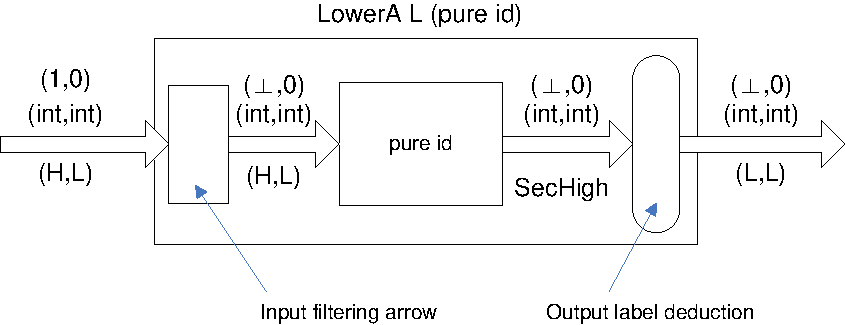
\includegraphics[scale=0.7]{lower.pdf} \\
%\captionof{figure}[Example of \co{lowerA}]{Example of \co{lowerA}}
%\end{center}

%
% Explain the diagram.
%
Assume we have a lattice of two labels, \co{L} and \co{H} where $\cod{L}\sqsubseteq \cod{H}$. A pair of 
integers that the first element has security label \co{H} and the second element has security label \co{L} are 
passed as the inputs.
Because the expected label is \co{L} in the \co{lowerA}, the first element of the pair becomes \co{undefined}
after passing through the input filter arrow. The implementation of input filter arrow is explained in
Sec.~\ref{chap5:lowerA:ifm}. The output security label of \co{pure} is \co{SecHigh}. However, the output
security type of the \co{lowerA} is derived from the output type. The output type is a pair of integers, so
the corresponding security label $(\cod{L},\cod{L})$ is generated. The implementation of the output label
deduction is explained in Sec.~\ref{chap5:lowerA:old}.
If the {\em undefined} value is used somewhere later in the program, the whole program
aborts immediately and no information can leak.

\subsection{Input Filtering Mechanism}
\label{chap5:lowerA:ifm}
The input filtering mechanism in \co{lowerA} is implemented by 
method \co{removeHigh} in type class \co{SecFilter}. Any type used as an input type in computations created by
\co{lowerA} requires an instance in the type class \co{SecFilter}. The implementations for integer, pair,
and reference are as following(in SecureFlow.hs):
\begin{Verbatim}[fontsize=\small]
class (Lattice l) => SecFilter s l t where
  removeHigh :: l -> (s l) -> t -> t

instance (Lattice l) => SecFilter SecType l Int where
  removeHigh l (SecLabel (Lab l')) t = 
               if label_leq l' l then t else undefined

instance (Lattice l, SecFilter SecType l a
         , SecFilter SecType l b) =>
           SecFilter SecType l (a,b) where
  removeHigh l (Pair lx ly) (x,y) = 
               (removeHigh l lx x, removeHigh l ly y)

instance (Lattice l, SecFilter SecType l a) =>
         SecFilter SecType l (SRef l a) where
  removeHigh l (Ref t (Lab l')) (MkSRef r fin fout) =
        if label_leq l' l
          then (MkSRef r ((removeHigh l t).fin) 
                           (\s x -> outFilter t s (fout s x)))
          else undefined

outFilter :: Lattice l => (SecType l) -> (SecType l) -> a -> a
outFilter s1 s2 a = if s2 `ml_leq` s1
                      then a
                      else error $ "Illegal reference write." 
\end{Verbatim}
Method \co{removeHigh} takes a lattice label \co{l}, a complex security type (\co{s~l}), and a value of 
type \co{t}. In the instance of \co{Int}, the security label is compared with \co{l}. If it is higher 
than \co{l}, \co{undefined} is returned. Otherwise, the same value is returned. This is the same for any 
data type that is protected by a lattice label.
When \co{removeHigh} is applied to a pair, \co{removeHigh} is applied to both elements
with the corresponding security types and values.

For reference, \co{removeHigh} compares the identity security label, $l'$, with expected security label, $l$. 
If $l'$ is higher than $l$, undefined is returned. Otherwise, \co{removeHigh} should applies to the content
of the reference. But even if the security label of the content is higher than $l$, the content of the 
reference cannot become \co{undefined} because it may be shared by other references. The \co{undefined} should
only be observed when the content is read out from the reference in discuss. All other references pointed to
the same content should be read normally. That is the reason that a {\em projection}
function is introduced in \co{SRef}. A partial evaluated function $(\cod{removeHigh}~l~t)$, which takes
a value and returns either the same value or \co{undefined}, is composed with the original projection function,
\co{p}. By this way, if the security label of the content is higher than expected, only the result of reading this
reference becomes \co{undefined}. 

On the other hand, a write protection function is also added in function \co{removeHigh} of references. Function
\co{outFilter} prevents the reference from written by any value that has security labels higher than \co{t}. 
The following program illustrates the necessity of the write protection function:
\begin{Verbatim}[fontsize=\small]
lowerA High (pure (\r -> r))
\end{Verbatim}
Assume a lattice has two labels, \co{Low} and \co{High}, and $\cod{Low}\sqsubseteq \cod{High}$. If a reference 
of security type $\cod{Low}~\mathbf{ref}^{\cod{Low}}$ is passed to the program above. The output 
security type becomes $\cod{High}~\mathbf{ref}^{\cod{High}}$. Then a value of security label \co{High} can
be written to the reference. However, if the content is shared with other references, the value with 
security label \co{High} may be read out as a value with security label \co{Low} from other references.

\subsection{Deduction of Output Security Label}
\label{chap5:lowerA:old}
Function $\rho$ in Figure~\ref{fig:deduce} is implemented by method \co{low} in type class \co{Downgrade}. 
Type class \co{Donwgrade} deduces security labels for a data type based on a value of
that type.
The definition of \co{Downgrade} and some instances are as following(in SecureFlow.hs): 
\begin{Verbatim}[fontsize=\small]
class (Lattice l) => Downgrade s l t where
  low :: l -> t -> (s l)

instance (Lattice l) => Downgrade SecType l Int where
  low l t = (SecLabel (Lab l))

instance (Lattice l, Downgrade SecType l a
         , Downgrade SecType l b) =>
           Downgrade SecType l (a,b) where
  low l (x,y) = (SecPair (low l x) (low l y))

instance (Lattice l, Dummy a, Downgrade SecType l a) =>
            Downgrade SecType l (SRef l a) where
  low l (MkSRef _ _ _) = (SecRef (low l (dummy::a)) (Lab l))
\end{Verbatim}
Type variable \co{s} is a complex security type based on a lattice \co{l}.
Method \co{low} takes a lattice label and a value of type \co{t}, and returns a corresponding security label 
for data type \co{t} with every label annotation being the lattice label.
In the instance of \co{Int}, a \co{SecLabel} with label annotation \co{l} is returned. 
In the instance of pair, a constructor \co{SecPair} is returned with method \co{low} applied again to both 
elements of the pair.
In the instance of reference types, function \co{low} is applied to deduce the security label of the content 
given a value which has the same type as the content, \co{a}.
Operator \co{dummy} belongs to type class \co{Dummy} and returns a value of type \co{a} in this case. 

The output type of a \co{FlowArrowRef} can be obtained in the type signature. 
Type class \co{DowngradeArrow} collects output types of {\em arrows} from
the type signatures(in SecureFlow.hs).
\begin{Verbatim}[fontsize=\small]
class (Lattice l, Arrow a) =>
      DowngradeArrow s l a b c where
  lowFlow :: l -> (a b c) -> (s l)

instance (Lattice l, Downgrade SecType l b
         , Downgrade SecType l c
         , Dummy b, Dummy c, Arrow a) =>
         DowngradeArrow SecType l a b c where
  lowFlow l t = low l (dummy::c)
\end{Verbatim}
Type variable \co{s} is a complex security type and variables \co{b} and \co{c} are the types of 
inputs and outputs of an {\em arrow} \co{a}.
Method \co{lowFlow} takes a lattice label and an {\em arrow}, and return a security type for the output.
In the instance of \co{SecType}, \co{lowFlow} returns an output security
type generated by method \co{low}, given an expected lattice label \co{l} and a value of type \co{c}.


\chapter{Adding Unification Inside of FlowHaskellRef }


\section{Unification}
\label{chap4:unification}

\newcommand{\unify}[1]{\stackrel{{#1}}{\sim}}
\newcommand{\ct}{c^l}
% Note
% Motivation
% Show UType and explain
% Show unification part of FlowArrowRef
% - how uniset is produced(find vars in flow and uniset, and rename, and then replace)
% Regulation when using unification variables to define new primitive

\begin{figure}[t]
\[
\alpha ::= \omega\ |\ \ell
\]
\caption{Extended lattice type}
\label{fig:unif:lt}
\end{figure}

\begin{figure}[t]
\[
\st\ ::=\ \alpha\ |\ \st\ \mathbf{ref}^{\alpha}\ |\ (\st,\st)\ |\ (\mathbf{either}\ \st\ \st)^{\alpha}\ 
        |\ \mathbf{high}\ |\ t
\]
\caption{Extended security type}
\label{fig:unif:st}
\end{figure}

\begin{figure}[t]
\[
\ell\unify{\emptyset} \ell\quad \quad \omega\unify{(\omega:=\alpha)} \alpha
\]
\caption{Unification of lattice}
\label{fig:unif:ul}
\end{figure}

\begin{figure}[t]
\[
  \begin{array}{c}
  \inference[]{\alpha_1\unify{U} \alpha_2}{\alpha_1\unify{U} \alpha_2} \quad
  
  \inference[]{\alpha_1\unify{U_1} \alpha_2 \quad U_1\sts{1}\unify{U_2} U_1\sts{2}}
              {\sts{1}\ \mathbf{ref}^{\alpha_1}\unify{U_2.U_1} \sts{2}\ \mathbf{ref}^{\alpha_2}} \quad

  \inference[]{\sts{1}\unify{U_1} \sts{3} \quad U_1\sts{2}\unify{U_2} U_1\sts{4}}
              {(\sts{1},\sts{2})\unify{U_2.U_1} (\sts{3},\sts{4}) }     \\ \\

  \inference[]{\alpha_1\unify{U_1} \alpha_2 \quad
               U_1\sts{1}\unify{U_2} U_1\sts{3} \quad {U_2}U_1\sts{2}\unify{U_3} {U_2}U_1\sts{4}}
              {(\mathbf{either}\ \sts{1}\ \sts{2})^{\alpha_1}\unify{U_3.U_2.U_1} 
               (\mathbf{either}\ \sts{3}\ \sts{4})^{\alpha_2}} \quad

  \inference[]{}
              {\mathbf{high}\unify{\emptyset} \mathbf{high}} \\ \\
  
  \inference[]{t \not\in \cod{FV}(\st)}
              {t\unify{t:=\st} \st}  \quad

  \inference[]{}
              {\mathbf{high}\unify{\emptyset} \top}  \quad

  \inference[]{}
              {\mathbf{high}\unify{\omega:=\top} \omega}  \\ \\

%  \inference[]{High\unify{U_1} \alpha \quad U_1High\unify{U_2} U_1\st}
%              {High\unify{U_2.U_1} \st\ ref^{\alpha} } \\ \\
%
  \inference[]{\mathbf{high}\unify{U_1} \sts{1} \quad U_1\mathbf{high}\unify{U_2} U_1\sts{2}}
              {\mathbf{high}\unify{U_2.U_1} (\sts{1},\sts{2})}  \quad

  \inference[]{\mathbf{high}\unify{U_1} \alpha \quad
               \mathbf{high}\unify{U_2} U_1\sts{1} \quad {U_2}U_1\mathbf{high}\unify{U_3} {U_2}U_1\sts{2}}
              {\mathbf{high}\unify{U_3.U_2.U_1} (\mathbf{either}\ \sts{1}\ \sts{2})^{\alpha}} \\ \\
  \end{array}
\]
\caption{Unification of security type}
\label{fig:unif:us}
\end{figure}

\begin{figure}[t]
\[
\ct ::= \ct\sqcap \ct\ |\ \ct\sqcup \ct\ |\ \mathbf{extr}\ \ct\ |\ \mathbf{fst}\ \ct\ |\ \mathbf{snd}\ \ct\        
        |\ \tagup\ l\ \ct\ |\ \decl\ l\ \ct\ |\ \st
\]
\caption{Unification constraint type}
\label{fig:unif:ct}
\end{figure}

\begin{figure}[t]
\[
 \begin{array}{c}
 \inference[]{\sts{1}\unify{U} \sts{2}}
             {\cod{Id}\ \sts{1}\unify{U} \cod{Id}\ \sts{2}} \quad
% \inference[]{|[\ct|]=\cod{Id}\ \st}
%              {v\unify{(v:=\st)} \ct}  \quad
 \inference[]{|[\ct|]\unify{U} \beta}
             {\ct\unify{U} \beta} \\ \\
 \end{array}
\]
\caption{Unification constraint elimination}
\label{fig:unif:ce}
\end{figure}

Primitive \co{createRef} takes a value and returns a reference, and the output security type 
, $\st~\mathbf{ref}^{\ell}$, contains two parts. 
One is a security type for the content and the other is a security label
for its own identity. The security type of the content is identical to the input
security type of \co{createRef} according to the type system in Figure~\ref{fig:reference:typesystem}. But how 
should the input security type be determined? In the framework
of FlowHaskell, the only feasible way is to ask the programmers to specify the security labels.
The following is an example using this approach:
\begin{Verbatim}[fontsize=\small]
pure (\_ -> 0) >>> createRef (SecLabel HIGH) LOW >>> 
readRef (SecLabel HIGH) LOW >>> ...
\end{Verbatim}
In \co{createRef}, the programmers are required to specify the security type of the input as well as
the security label of the identity. Similar in \co{readRef}, both the security types of the content and
the identity need to be specified. In many cases, however, the creation and reading of a reference reside in
very different parts of a program, and the programmers have to specify the right security types. This is
not only tedious but error-prone. Consider a small error in \co{readRef} as following:
\begin{Verbatim}[fontsize=\small]
pure (\_ -> 0) >>> createRef (SecLabel HIGH) LOW >>>
readRef (SecLabel LOW) LOW >>> ...
\end{Verbatim}
The \co{HIGH} content of the reference becomes \co{LOW} due to a mistake by specifying wrong security type. 
To avoid this kind of mistakes, a new mechanism to pass security types through computation 
is demanded. Unification is adopted in FlowHaskellRef to resolve the limitation.

The main idea is to extend the ability of passing security types in the \co{flow} field 
of \co{FlowArrowRef}. Unification variables can be used to define primitives and are aimed to
receive security types from previous computations when combined by {\em arrows} combinators.
To certify a computation, all the variables are unified first and the computation is 
certified as before.

\subsection{Unification Types}
Two kinds of unification variables are required. One can be unified with a lattice label and the other
is used to  unify with a complex security type. In Figure~\ref{fig:unif:lt} a new constructor, variable $\omega$,
is extended in the original lattice type. It is implemented by a new data type \co{Label} as following
(in Lattice.hs):
\begin{Verbatim}[fontsize=\small]
data Label l = Lab l | LVar String
\end{Verbatim}
To unify with a complex security type, $\st$ has a new constructor, $t$, for unification variable, as in 
Figure~\ref{fig:unif:st}. Data type \co{SecType} is modified to reflect the new design(in Lattice.hs).
\begin{Verbatim}[fontsize=\small]
data SecType l = SecLabel (Label l) 
               | Ref (SecType l) (Label l)
               | SecVar String
               | ...
\end{Verbatim}
Constructors not showed above are the same as before.

The unification semantics for a lattice type is depicted in Figure~\ref{fig:unif:ul}. When two lattice labels
unify with each other, they should be identical. If one is a variable, a new unification
result is generated. Figure~\ref{fig:unif:us} shows the unification semantics for $\st$. 
Symbol $\unify{U}$ denotes a unification that produces some unification results, $U$. A unification
result along with a security type, $U\st$, updates the security type, $\st$, according to the unification
result, $U$. If more than one unification result are produced, the final unification result is the 
composition of all results in the same order as they are generated. Notice that there is no rule to
unify a $\mathbf{high}$ and a ($\st~\mathbf{ref}^\alpha$). The reason is the security label of the content
of a reference is invariant in the sub-typing relation in Figure~\ref{fig:subtyping}. Unifying with
$\mathbf{high}$ may break the relation.

Many operators takes security types and are required to generate constraints in \co{FlowArrowRef}, but
they can only defined for security types which contain no unification variables. 
Therefore, those operations should be retained and performed until all variables inside of the involving
security types are resolved. A new type called unification constraint, as in Figure~\ref{fig:unif:ct}, 
represents those operators and postpones the operations until all variables are unified to some
security types.
Those constraints are implemented by data type \co{U}(in Unification.hs):
\begin{Verbatim}[fontsize=\small]
data U s = Meet (U s) (U s)
         | Join (U s) (U s)
         | LExtr (U s)
         | Fst (U s)
         | Snd (U s)
         | Tag (U s) (U s)
         | Decl (U s) (U s) (U s)
         | Id s
\end{Verbatim}
Type variable \co{s} is \co{SecType} in our case. 
Constraints $\sqcap$ and $\sqcup$ correspond to the \co{Meet} and the \co{Join} constructors. 
The operations are performed in method \co{ml\_meet} and \co{ml\_join} of \co{SecType} respectively. 
Constraint $\mathbf{extr}$ is implemented by \co{LExtr} and resolved by method \co{mextract}.
Constraint $\mathbf{fst}$ and $\mathbf{snd}$ returns the first and the second element of a pair respectively.
Constraint $\tagup$ is implemented by constructor \co{Tag} and performed by method \co{ml\_tag}.
Constraint $\decl$ corresponds to constructor \co{Decl} and resolved by method \co{ml\_decl}. One more
parameter in \co{Decl} than those in constraint $\decl$ is due to implementation issues about \co{SecHigh}. 
It is a \co{SecType} with expected security labels and returned as a result when \co{SecHigh} is encountered
in the first argument.
The last constraint is just a \co{SecType} and implemented by constructor \co{Id}.
Besides, any \co{Label} is wrapped in a \co{SecLabel} constructor so both data type \co{SecType} and data type 
\co{Label} can share the same constraint type. For example, a label (\co{Lab} \co{l}) in constraint \co{U} 
becomes  (\co{Id} (\co{SecLabel} (\co{Lab} \co{l}))).

The unification semantics for unification constraint is depicted in Figure~\ref{fig:unif:ce}. When two constraints
are both \co{SecType}s, they are unified according to the unification semantics of $\st$. The second rule says
if a constraint contains no variable, the corresponding operation is performed before unification, 
denoted by symbol $|[|]$. Otherwise, the constraint is put back to the unification set and try again later.

\subsection{Unification in FlowArrowRef}
\label{chap4:unification:flowarrowref}
% show real definition of FlowArrow and FlowArrowRef
% explain new Flow definition
% explain usage of uniset
% explain alpha conversion
% explain binding operators with unification
To extend unification in FlowHaskellRef, new fields to handle unification variables are required.
The following is the complete definition of \co{FlowArrowRef}(in FlowArrowRef.hs):
\begin{Verbatim}[fontsize=\small]
data FlowArrowRef l a b c = 
    FARef { computation :: ((SecType l) -> (SecType l)) 
                           -> a b c
          , flow        :: Flow (SecType l)
          , constraints :: [Constraint (SecType l)]
          , gconstraints:: [GConstraint (SecType l)]
          , pc          :: (SecType l)
          , uniset      :: [(U (SecType l), U (SecType l))]
          }

data Flow l = Trans l l 
\end{Verbatim}
Field \co{computation} becomes a function that accepts a substitution function and returns an underlying
{\em arrow} computation. A substitution function takes a \co{SecType} and returns a new \co{SecType} with some 
internal variables replaced with other \co{SecType}s.
The reason of introducing a substitution function is explained in Sec.~\ref{chap5:lower:implement}.
New definition of \co{Flow} removes constructor \co{Flat} which loses constructor information of a
security type. A new field, \co{uniset}, contains a list of pairs of constraint types which are aimed 
to be unified.
Field \co{pc} becomes \co{SecType} rather than a lattice type. This is due to implementation issues that 
security types in field \co{uniset} should have a uniform type.
The interpretation of \co{pc} remains the same.

When defining new primitives with unification, variables normally appear in the input security type 
because it is the only place to receive information from previous computations.
Those variables can also be used to define constraints within the 
same \co{FlowArrowRef}. But when combining two \co{FlowArrowRef} computations via arrow combinators,
it is possible that two computations have variables with identical names but are actually distinct.
Those variables are likely to be inconsistent and cannot be resolved to a single value in unification 
algorithm. As a result, every variable is renamed to a distinct name in {\em arrows} combinators. 
To collect all variables in a \co{FlowArrowRef} computation, it is sufficient to collect variables in the field
\co{flow} and \co{uniset}. New variables must appear either in field \co{flow} or field
\co{uniset} so that they can be unified to a value afterward. 
After all variables are collected, a substitution containing a list of old name and new name pairs are
generated.
Then, variables in all fields are replaced with their new names according to the substitution.

Since security types are passed through field \co{flow} by unification variables,
combinators need to compute new \co{flow}s that pass 
security types as well as fulfill the type system described in Sec.~\ref{chap4:flowarrowref:typesystem}.
In the rest of this section, we explain how each combinator produces flow security types in the presence
of unification variables, and show that they obey the type system.

Combinator \co{pure} defines its \co{flow} to be ($t~->~\mathbf{high}$) which implements the type system
directly(in FlowArrowRef.hs).
\begin{Verbatim}[fontsize=\small]
pure f = FA { ...
              flow = Trans (SecVar "x0") SecHigh
              ... }
\end{Verbatim}
The \co{flow} of combinator (\arrowop{>}) is defined by the following function(in FlowArrowRef.hs):
\begin{Verbatim}[fontsize=\small]
flow_seq :: Lattice l => 
            Flow (SecType l) -> Flow (SecType l)
            -> ( Flow (SecType l)
               , [Constraint (SecType l)]
               , [(U (SecType l),U (SecType l))])
flow_seq (Trans s1 s2) (Trans s3 s4)= (Trans s1 s4, c,u)
  where
  (c,u) = seqFlow s2 s3

seqFlow s2 s3 =
  case (s2,s3) of
    (t1@(SecVar _), t2) -> if (hasVarSecType t2)
                             then ([],[(Id t1,Id t2)])
                             else ([LEQ t1 t2], [])
    ...
    (SecPair t1 r1, SecPair t2 r2) -> let (ct,ut) = seqFlow t1 t2
                                          (cr,ur) = seqFlow r1 r2
                                      in (ct++cr,ut++ur)
    ...
\end{Verbatim}
Given input and output security types of two \co{FlowArrowRef}s, function \co{flow\_seq} returns a new \co{flow}
as (\co{Trans} \co{s1} \co{s4}).
Function \co{seqFlow} takes two security types, \co{s2} and \co{s3}, and generates additional constraints and 
unification pairs. 
As in the first case pattern matching of \co{seqFlow}, if \co{s2} is a variable and \co{s3} contains no variable, 
a new constraint $\cod{s2}\sqsubseteq \cod{s3}$ is generated. This is the same as in the type system.
On the other hand, if \co{s3} contains variables, it is aimed to receive information from \co{s2}, so \co{s3}
should be unified with \co{s2}. This means $\cod{s2}=\cod{s3}$ and the constraint 
$\cod{s2}\sqsubseteq \cod{s3}$ is satisfied implicitly. 
If \co{s2} and \co{s3} contains structure information, the sub-components of them are again compared by \co{seqFlow}.
For example, if both \co{s2} and \co{s3} are \co{SecPair}, the first and the second components of them are
compared respectively. 
This fine-grained comparison still obey the constraint $\cod{s2}\sqsubseteq \cod{s3}$ in the type system.

For combinators \co{first}, \co{second}, and (\arrowop{*}), the new flow security type is implemented by 
function \co{flow\_pair}(in FlowArrowRef.hs). 
\begin{Verbatim}[fontsize=\small]
flow_pair :: Lattice l => Flow (SecType l) 
             -> Flow (SecType l) -> Flow (SecType l)
flow_pair (Trans s1 s2) (Trans s3 s4) = 
                Trans (SecPair s1 s3) (SecPair s2 s4)
\end{Verbatim}
It simply puts input and output security types in pair constructors respectively.
For combinator (\arrowop{\&}), more analyses are required 
in \co{flow\_diverge}(in FlowArrowRef.hs).
\begin{Verbatim}[fontsize=\small]
flow_diverge :: Lattice l => 
     Flow (SecType l) -> Flow (SecType l)
     -> ( Flow (SecType l)
        , [Constraint (SecType l)]
        , [(U (SecType l), U (SecType l))])
flow_diverge (Trans s1 s2) (Trans s1' s2') =
  let (in_flow, cons, us) = meetInFlow s1 s1' in
  (Trans in_flow out_flow, cons, us)
  where
  out_flow = (Pair s2 s2')

meetInFlow s1 s2 =
  case (s1,s2) of
    (t1@(SecVar _), t2@(SecVar _)) -> (t1, [], [(Id t1,Id t2)])
    (t1@(SecVar _), t2) -> if hasVarSecType t2
                             then (t1, [], [(Id t1,Id t2)])
                             else (t1, [LEQ t1 t2], [])
    ...
    (SecLabel l1, SecLabel l2) -> 
                let (l' , cons, us) = meetInFlowLabel l1 l2
                in (SecLabel l', cons, us)
    (Pair s1 t1, Pair s2 t2) -> 
                let (s', scons, sus) = meetInFlow s1 s2
                    (t', tcons, tus) = meetInFlow t1 t2
                in (Pair s' t', scons++tcons, sus++tus)
    ...

meetInFlowLabel k1 k2 =
 case (k1,k2) of
  (l1@(LVar _), l2@(LVar _)) -> 
                 (l1, [], [(Id (SecLabel l1),Id (SecLabel l2))])
  (l1@(LVar _), l2) -> (l1,[LEQ (SecLabel l1) (SecLabel l2)],[])
  (l1, l2@(LVar _)) -> (l2,[LEQ (SecLabel l2) (SecLabel l1)],[])
  (Lab l1, Lab l2) -> (Lab (label_meet l1 l2), [], [])
\end{Verbatim}
According to the type system, the new input security type is the meet of the two original input security types.
Function \co{meetInFlow} traverses and compares two original input security types simultaneously, 
and produces a security type that approximates the type system.
If two variables are compared, since they both expect to receive the security types from previous computation,
they should be identical. Thus, any of them can represent new input security type and a unification pair is 
generated to ensure that they are the same.
In the case that only one input security types is a variable, if the other security type contains no variable,
the variable is regarded as new input security type. A constraint \co{LEQ} is required to guarantee that the 
resulting security type is the meet of the two input security types. 
However, if the other security type contains variables, an approximation is made to force the two security
types are the same. In this way, any certified program still obeys the type system. 
The second pattern matching of the case statement in function \co{meetInFlow} implements the idea described above.
A constraint (\co{LEQ} \co{t1} \co{t2}) is generated in the case that \co{t2} contains no variable.
In the other case, a unification pair of \co{t1} and \co{t2} is generated to ensure that they are identical.
This approximation rejects some legal programs. One way to avoid this is to provide unification 
constraints to extract sub-component of each security type constructors, such as \co{Fst} and \co{Snd} for pairs.
Thus, the meet of the two input security types can be precisely
produced after all variables are unified. This is one of the future work of FlowHaskellRef.
In the case that both of input security types contain no variable, function \co{meetInFlow} and 
function \co{meetInFlowLabel} is applied to the sub-components of the security types.
Function \co{meetInFlowLabel} is similar to function \co{meetInFlow} but compares two security labels.

Function \co{flow\_either} defines
flow for \co{left}, \co{right}, and (\arrowop{+})(in FlowArrowRef.hs).
\begin{Verbatim}[fontsize=\small]
flow_either (Trans s1 s2) (Trans s3 s4) = 
               Trans (SecEither s1 s3 (LVar "x0")) 
                     (SecEither s2 s4 (LVar "x0"))
\end{Verbatim}
A lattice label for the identity of \co{SecEither} is received from previous computations and passed
as the identity security label of output \co{SecEither}. It implements the type system directly.

Function \co{flow\_converge} returns flow of ($|||$) and a list of unification
pairs(in FlowArrowRef.hs):
\begin{Verbatim}[fontsize=\small]
flow_converge :: Lattice l => 
                 Flow (SecType l) -> Flow (SecType l)
                 -> ( Flow (SecType l)
                    , [(U (SecType l),U (SecType l))])
flow_converge (Trans s1 s2) (Trans s1' s2') =
  let l = (LVar "x0") in
  let s_out = (SecVar "x1") in
  (Trans (SecEither s1 s1' l) s_out
  ,[(Id s_out, Tag (Join (Id s2) (Id s2')) (Id (SecLabel l)))])
\end{Verbatim}
The identity label of input security label \co{SecEither} is a variable to receive a lattice label
from previous computations.
The resulting output security type is the result of applying function $\tagup$ to the join of 
two original output security types.

%Method \co{loop} in \co{ArrowLoop} takes an {\em arrow} whose input and output are both pairs, and 
%returns a new {\em arrow}. The new input is the first element of the input, and the new output is
%the first element of the output. The second element of the output is taken as the second
%element of the input to form a feedback computation.
%Function \co{flow\_loop} takes the \co{flow} of the input {\em arrow} and returns a new \co{flow} 
%and an additional constraint.(in FlowArrowRef.hs)
%\begin{Verbatim}
%flow_loop :: Lattice l => Flow (UType l)
%             -> (Flow (UType l)
%                ,[Constraint (UType l)])
%flow_loop (Trans a b) = 
%    (Trans (UFst a) (UFst b)
%    ,[LEQ (USnd b) (USnd a)]) 
%\end{Verbatim}
%New \co{flow} is a flow from the first element of the input security label to the first element of the
%output security label. A new constraint is required because the feedback introduced in \co{loop}.

Except field \co{flow}, other fields of \co{FlowArrowRef} implement the type system 
in Sec.~\ref{chap4:flowarrowref:typesystem} directly, although the enforcement of the type system are 
postponed until unification variables are unified successfully.

\subsection{Defining New Primitives}
% no new variables has 'a' as first char.
% new variables only introduced in flow field.
New primitives of \co{FlowArrowRef} may take advantages of unification.
Unification variables provide a possibility of receiving information from 
other computations.
However, there are two rules which should be strictly obeyed to guarantee success of unification
algorithm.
\begin{enumerate}
\item Names of new variables cannot begin with a character 'a' and followed by an integer.
\item New variables in a primitive must appear either in input security types or unification set.
\end{enumerate}
First rule comes from the fact that variables are renamed to the format internally. A new variable may 
have a name collision with existing ones if not named properly. 
If a variable violates the second rule, the variable cannot be resolved to a security type and the
unification algorithm will fail.


\section{Implementation of \co{lowerA}}
\label{chap5:lower:implement}
With unification added to \co{FlowArrowRef}, we are now ready to explain the implementation
of \co{lowerA}(in FlowArrowRef.hs):
\begin{Verbatim}[fontsize=\small]
lowerA :: (Lattice l, Arrow ar,
         Downgrade SecType l a, Downgrade SecType l b,
         Dummy a, Dummy b, SecFilter SecType l a,
         DowngradeArrow SecType l (FlowArrowRef l ar) a b)
        =>
          l -> FlowArrowRef l ar a b -> FlowArrowRef l ar a b
lowerA level fa@(FARef com' (Trans s_in' _) cons' 
                          gcons' pc' uniset') =
   let flow_out = (lowFlow level fa) in
   let inputFilter upd = 
         pure (\i -> (removeHigh level (upd s_in') i)) in
   FARef { computation = (\upd -> (inputFilter upd) 
                                  >>> (com' upd))
         , flow = Trans s_in' flow_out
         , constraints = [LEQ (SecLabel (Lab label_top)) pc'] 
                         ++ cons'
         , gconstraints = [GLLEQS (SecLabel (Lab level)) s_in'] 
                          ++ gcons'
         , pc = (SecLabel (Lab label_top))
         , uniset = uniset'
         }
\end{Verbatim}
Combinator \co{lowerA} takes a lattice label, \co{level}, and a \co{FlowArrowRef}, \co{fa}.
The new \co{pc} is $\top$ and the new constraint in field \co{constraintsRef} requires \co{pc'} to
be $\top$ as well.
The reason is that \co{lowerA} is developed to alleviate the limitation of \co{pure}, and computations involves
reference manipulations should be kept out of \co{lowerA}. Otherwise, the security type of a reference's
content may become inconsistent because \co{lowerA} only generate output security types based on the output
type.

Method \co{lowFlow} is applied to the lattice label \co{level} and computation \co{fa},
and returns a derived output security label \co{flow\_out}.
Function \co{inputFilter} defines the input filter function via \co{pure} of underlying {\em arrow} computation,
and it filters the inputs by sequenced before the desired computation \co{com'}.
Input security label \co{s\_in'} in \co{inputFilter} may be a variable and can only be resolved to a value 
after unification. 
Moreover, during the construction of a \co{FlowArrowRef} program, \co{s\_in'} may be renamed several times 
in combinators of \co{FlowArrowRef}. 
Thus, a substitution function, called \co{upd}, is taken in function \co{inputFilter}. 
A substitution function takes a security type and returns a new security type which is similar to the input but
with some variables inside replaced by other security types or variables. Function \co{upd} is applied to input security
type \co{s\_in'} and the result is a security type without variables.
Because the substitution function is known only from outside a computation, the definition
of field \co{computation} is adapted to take a substitution function and returns an underlying {\em arrows} computation,
as described in Sec.~\ref{chap4:unification:flowarrowref}.

The substitution function is constructed in {\em arrows} combinators. The following is an example of combinator
(\arrowop{>})(in FlowArrowRef.hs):
\begin{Verbatim}[fontsize=\small]
a1@(FA c1 f1 t1 g1 pc1 u1) >>> a2@(FA c2 f2 t2 g2 pc2 u2) =
     ...
     let (sub1, sub2, _) = (make_sub a1 a2 []) in
     let (f,c,u) = flow_seq (replace_flow sub1 f1) 
                            (replace_flow sub2 f2) in
     FARef{
     computation = 
         (\upd -> c1 (upd.(replaceSecType sub1)) >>>
                  c2 (upd.(replaceSecType sub2)))
     ...
     }

replaceSecType :: Lattice l => [(SecType l, SecType l)] 
                  -> SecType l -> SecType l
\end{Verbatim}
Function \co{make\_sub} collects all variables in \co{FlowArrowRef} \co{a1} and \co{a2}, and returns 
substitutions \co{sub1} and \co{sub2}. A substitution is a list of old variable name and new variable name pair. 
Function \co{replaceSecType} takes a substitution and becomes
a substitution function defined in the paragraph above. In field \co{computation}, a new substitution 
function (\co{replaceSecType} \co{sub1}), for instance,  
is composed with the substitution function
passed from outside. By this substitution function composition, a variable inside a computation 
performs all renaming in the same order as other variables in other fields. At top level, 
a substitution function that substitute variables according to the unification result is passed. 
It substitutes a variable to a security type containing no variables.

\chapter{Case Study of FlowHaskellRef}

In the case study, a cryptographic protocol between a client card, an ATM, and a bank is implemented
to show that FlowHaskellRef can be used to build bigger applications. The case study is revised
from Tse and Washburn's work~\cite{Tse:Washburn:jif}, which is a case study for Jif~\cite{jif}.

\section{Cryptographic Protocol}
The scenario of the case study is as following.
A bank card is inserted in an ATM machine and two messages are exchanged between the ATM 
machine and a bank server for authentication. If the authentication succeeds, another
two messages are exchanged for transaction. In real situation, messages are delivered over public
networks. To guarantee confidentiality, they are encrypted before sent. In the case study, we
simulate the public networks as IO monad for simplicity and each message passing in the IO monad is 
public and should be encrypted. Besides, only the protocol involving security data is implemented.
Key generation and a database in the bank server, which appear in 
Tse and Washburn's work~\cite{Tse:Washburn:jif}, are skipped.

\subsection{Protocols}
The protocol contains the following four messages.
\begin{enumerate}
\item \textbf{Authentication request} The message is from an ATM to a bank server and contains two data.
      One is the account number read from a client card, $\cod{id}_c$, and the other is a nonce generated by the ATM,
      $\cod{n}_a$. The message is encrypted with the public key of the bank, $\cod{k}_b$, and as following:
      \[
         \{~\cod{id}_c,~\cod{n}_a~\}_{\cod{k}_b}
      \]
\item \textbf{Authentication response} When a authentication request is received by a bank 
      server, it is decrypted with the private key of the bank. A session key, \co{s}, and a bank nonce, 
      $\cod{n}_b$, are generated by the bank server. Along with the ATM nonce received in the authentication
      request, the authentication response is encrypted with the public key of the client, $\cod{k}_c$,
      and sent back to the ATM. The message is as following:
      \[
         \{~\cod{s},~\cod{n}_a,~\cod{n}_b\}_{\cod{k}_c}
      \]
\item \textbf{Transaction request} The ATM retrieves the private key of the client, $\cod{p}_c$, with a correct 
      password, and it is used to decrypt the authentication response. The ATM nonce in the decrypted
      message is verified to be the same as the one sent in the authentication request. 
      A transaction, \co{tran}, contains the account number, type of action(deposit or withdraw, \co{act}),
      amount(\co{mnt}), and a new ATM nonce($\cod{n}_a$). A signature, \co{sig}, is obtained by signing 
      \co{tran} with the private key of the client. Together with $\cod{n}_b$ received in the authentication
      response and the new ATM nonce $\cod{n}_a$, the transaction request is encrypted with the session key 
      also received in the authentication
      response and sent to the bank server. 
      \[
        \begin{array}{l}
          \cod{tran}~=~(~\cod{id}_c,~\cod{act},~\cod{mnt},~\cod{n}_a) \\
          \cod{sig}~=~\{~\cod{tran}~\}_{\cod{p}_c} \\
          \{~\cod{tran},~\cod{sig},~\cod{n}_a,~\cod{n}_b~\}_\cod{s} \\
        \end{array}
      \]
\item \textbf{Transaction response} Transaction request is decrypted with the session key. The bank nonce
      is verified to be the same as the one sent in the authentication response. Then a new bank nonce,
      $\cod{n}_b$, is generated. Along with the ATM nonce received in the request and a response(transaction
      complete or failure, \co{res}), the transaction response is encrypted with the same session key and
      sent to the ATM.
      The message is as following:
      \[
         \{~\cod{res},~\cod{n}_a,~\cod{n}_b~\}_\cod{s} \\
      \]
\end{enumerate}

\subsection{Cryptographic Library} 
The Haskell cryptographic library is adopted to encrypt and decrypt messages described in the previous section.
Cryptosystem RSA is chosen for public-key encryption and signature signing, and the encryption and 
decryption primitives are in module \co{Codec.Encryption.RSA}.
Advanced Encryption Standard(AES) is used for symmetric-key encryption. The required primitives are in module
\co{Codec.Encryption.AES}.


\section{Implementation in FlowHaskellRef}
In the bank system simulation, a bank lattice is developed to represent different security levels of data in the program. 
A set of trusted computing base is identified, and then we show how information flow policies are enforced to
achieve the security goals of the simulation. The rest of the section explains each topic in details.

\subsection{Bank Lattice}
\begin{figure}[t]

%\begin{center}
%\begin{picture}(160,85)
% \put(68,0){BOTTOM}
% \put(75,75){TOP}
% \put(25,45){CLIENT}
% \put(115,55){BANK}
% \put(80,30){ATM\_BANK}
% \put(140,30){BANK\_ATM}
% \thicklines
% \drawline(85,73)(40,55)   %TOP -> CLIENT
% \drawline(85,73)(125,65)  %TOP -> BANK
% \drawline(127,53)(100,40) %BANK -> ATM_BANK
% \drawline(127,53)(160,40) %BANK -> BANK_ATM
% \drawline(40,43)(86,10)   %CLIENT -> BOTTOM
% \drawline(100,28)(86,10)  %ATM_BANK -> BOTTOM
% \drawline(160,28)(86,10)  %BANK_ATM -> BOTTOM
%\end{picture}
%\end{center}

%\begin{center}
%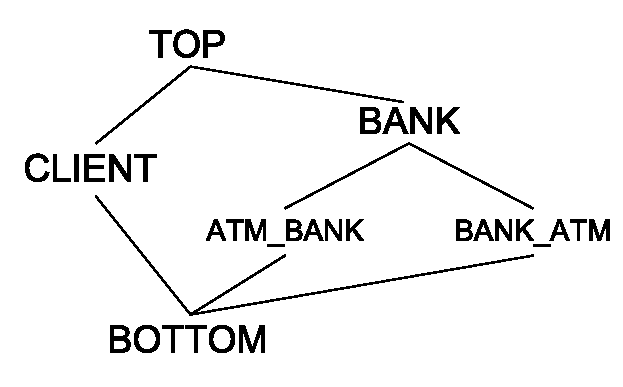
\includegraphics[scale=0.5]{bank.pdf} \\
%\end{center}

\caption{Bank lattice}
\label{fig:banklattice}
\end{figure}
A data type \co{BankLabel} is defined in the case study and its elements form a lattice illustrated 
in Figure~\ref{fig:banklattice}.
Label \co{CLIENT} classifies data that belong to a client card, e.g. the private key of the client.
Label \co{BANK} classifies data that belong to the ATM and the bank server. For instance, session keys used in
AES cryptosystem are
protected by \co{BANK}. Label \co{ATM\_BANK} classifies data that are generated in the ATM or sent from the ATM
to the bank server. Label \co{BANK\_ATM}, in contrast, classifies data that are generated in the bank server or
sent from the bank server to the ATM.
For example, the ATM nonce generated in the ATM is protected by \co{ATM\_BANK},
while the ATM nonce received from the bank server in the ATM is protected by \co{BANK\_ATM}. 
All data that are released to IO monad are public and thus protected by label \co{BOTTOM}.
Label \co{TOP} is introduced to complete the lattice.

\subsection{Trusted Computing Base}
\label{chap6:banksystem:tcb}
In the bank system simulation, secure programs constructed in FlowHaskellRef have type (\co{Protected} \co{c}).
The definition of \co{Protected} is as following:
\[
\cod{type}~\cod{Protected}~\cod{c}~=~\cod{FlowArrowRef}~\cod{BankLabel}~\cod{ArrowRef}~()~\cod{c}
\]
Each secure program receives a unit and returns a value of type \co{c}. Data type \co{ArrowRef} is an {\em arrow}
that supports computation in the IO monad.

Function \co{main} simulates network as the IO monad for message passing and is as following(in BankTCB.hs):
\begin{Verbatim}[fontsize=\small]
main =
  do -- Declare reference and protect them
     atm_ATMNonce    <- getNewRef ATM_BANK (1::Int)
     atm_BankNonce   <- getNewRef BANK_ATM (2::Int)
     atm_SessionKey  <- getNewRef BANK (3::Word128)
     bank_ATMNonce   <- getNewRef ATM_BANK (4::Int)
     bank_BankNonce  <- getNewRef BANK_ATM (5::Int)
     bank_SessionKey <- getNewRef BANK bankSeKey     
     -- Protocol begins
     auth_req <- atm_authRequest atm_ATMNonce (PR BANK)
     auth_res <- bank_authResponse auth_req bank_ATMNonce 
                   bank_BankNonce bank_SessionKey (PR BANK)
     tran_req <- atm_tranRequest auth_res atm_ATMNonce 
                   atm_BankNonce atm_SessionKey
                   (client_getPriKey (PR CLIENT)) (PR BANK)
     tran_res <- bank_tranResponse tran_req bank_ATMNonce 
                   bank_BankNonce bank_SessionKey (PR BANK)
     atm_resultProcess tran_res
     return ()
  where
  bankSeKey = (0x06a9214036b8a15b512e03d534120006::Word128)
  getNewRef l init =
    do ref <- createMRef init
       let pref = tagRef l >>> lowerA l (pure (\() -> ref))
       return pref
\end{Verbatim}
References are used to store all sorts of data, such as keys, ATM nonces, and bank nonces. In the first
part of \co{main}, they are created and protected by appropriate labels. This part belongs to TCB.
In the second part of \co{main},
four messages are passed in the IO monad. For each procedure, required data references and a privilege are given.
The dispatch of references and privileges belongs to TCB. Function \co{main} is separated in module \co{BankTCB}
because the constructor of privilege, \co{PR}, is only in scope in this module. 
As a result, the programs built in other modules can only declassify data with the privilege
given in the TCB.

To run a FlowHaskellRef program in the IO monad, function \co{expose} must be used to release the program from
type \co{Protected} to type \co{IO}.
The definition is as following(in BankSystem.hs):
\begin{Verbatim}[fontsize=\small]
expose :: (Privilege BankLabel) -> SecType BankLabel 
          -> Protected c -> IO c
expose p r t = runArrowRef (certifyRef (SecLabel (Lab label_bottom)) 
                                       (ml_bottom r) p t) ()
\end{Verbatim}
Function \co{expose} certifies a program with an input security type $\bot$ and an output security
type having the same structure as \co{r} but with every security label being $\bot$.

\subsection{Security Assumptions}
The following are the security assumptions of the bank system simulation.
\begin{itemize}
\item Data in the IO monad of function \co{main} are public and cannot be trusted.
\item The client's password is well-protected and can not be obtained by unauthorized people.
\item RSA and AES cryptosystems are unbreakable within tolerable computation power and time.
\item Programs mentioned in Sec.~\ref{chap6:banksystem:tcb} is trusted.
\end{itemize}

\subsection{Confidentiality of Bank System}
Function \co{expose} must be used to certify a FlowHaskellRef program before executing and releasing the 
result in the IO monad. It expects the output security
type with all security labels being $\bot$, which means the result is public. This satisfies the first 
security assumption that the IO monad cannot be trusted.

There are thirteen \co{declassifyRef} statements appearing in the program. The following justifies that each use 
of \co{declassifyRef} is adequate. They are organized by the functions using them.
\begin{itemize}
\item Function \textbf{encryptRSA}(in BankSystem.hs) \\
      The data declassified to $\bot$ is encrypted by RSA cryptosystem. According to the security
      assumptions, the data is secure by itself.
\begin{Verbatim}[fontsize=\small]
encryptRSA l_owner p_owner req key =
  let enreq = req >>> tagRef l_owner >>> 
              lowerA l_owner 
                (pure (\plain -> RSA.encrypt key plain))
              >>> declassifyRef BOTTOM 
  ...
\end{Verbatim}

\item Function \textbf{client\_getPriKey}(in BankTCB.hs) \\
      The ownership of the private key is transferred from \co{CLIENT} to \co{BANK} if a correct password
      is provided. According to the security assumptions, the password is secure, so the declassification
      is proper.
\begin{Verbatim}[fontsize=\small]
ient_getPriKey pr p =
  if p /= clientPW
    then return Nothing
    else let key = clientPriKey >>> declassifyRef BOTTOM in
         do pri <- expose pr (SecLabel (Lab BOTTOM)) key
            return $ Just (tagRef BANK >>> 
             lowerA BANK (pure (\() -> (clientModulus,pri))))
\end{Verbatim}

\item Function \textbf{atm\_AuthResDecrypt}(in BankSystem.hs) \\
      There are two declassification statements in the function. The message received from the bank server is decrypted with
      the private key of the client. The private key \co{pk} is protected by \co{BANK}, so the first declassification 
      is required to downgrade the decrypted data to \co{BANK\_ATM}, a proper label for data received from the 
      bank server. In the second declassification, the result of verifying the equality of two ATM nonce's is made
      public. This is the necessary one-bit information for the procedure to continue or to stop and reveals no 
      other information, so the declassification is adequate.
\begin{Verbatim}[fontsize=\small]
...
let dres = 
    pk >>>
    lowerA BANK (pure (\key -> RSA.decrypt key res)) >>>
    declassifyRef BANK_ATM >>>
    ...
    lowerA BANK (pure (\(a,b) -> if a == b then True else False))
    ...
    >>> declassifyRef BOTTOM
...
\end{Verbatim}

\item Function \textbf{atm\_getSignature}(in BankSystem.hs) \\
      The password of the client, \co{ppw}, is protected by \co{BANK}. 
      Declassification is required to retrieve the private key
      of the client to sign the signature. The password is public only inside this function and
      should not be returned. Therefore, the declassification is proper.
\begin{Verbatim}[fontsize=\small]
atm_getSignature tran client_prikey ppw priv =
  do let password = ppw >>> declassifyRef BOTTOM
     pw <- expose priv (SecLabel (Lab BOTTOM)) password
     cpri <- client_prikey pw
     ...
\end{Verbatim}

\item Function \textbf{atm\_buildTranRequest}(in BankSystem.hs) \\
      The declassified data is encrypted by AES cryptosystem and is secure according to
      the security assumptions. Thus, the declassification is adequate.
\begin{Verbatim}[fontsize=\small]
...
lowerA BANK (pure (\(c,key) -> 
  cbc AES.encrypt sessionIV key (pkcs5 c) )) >>>
declassifyRef BOTTOM
...
\end{Verbatim}

\item Function \textbf{bank\_TranDecrypt}(in BankSystem.hs) \\
      There are two declassification statements in the function. The first one declassifies data that are decrypted with
      the session key to \co{ATM\_BANK}. The justification is the same as the first declassification in function
      \textbf{atm\_AuthResDecrypt}. The second declassification declassifies the content of the message but
      they are protected separately right away in the \co{return} statement. Therefore, the declassification
      is adequate.
\begin{Verbatim}[fontsize=\small]
...
let 
dtran = sessionKey >>> readRef (SecLabel (Lab BANK)) >>>
        lowerA BANK (pure (\key -> 
         unPkcs5 (unCbc AES.decrypt sessionIV key tran) ))
        >>> declassifyRef ATM_BANK >>>
        ...
        >>> declassifyRef BOTTOM
(trans,(sig,(atm_n,bank_n))) <- exposeL priv dtran
return (protect trans, protect sig, 
        protect atm_n, protect bank_n)
where
protect t = tagRef ATM_BANK >>> 
            lowerA ATM_BANK (pure (\( -> t))
\end{Verbatim}

\item Function \textbf{bank\_checkBankNounce}(in BankSystem.hs) \\
      One-bit information about the bank nonces' equality is released. This piece of information is
      necessary for the procedure to continue or to stop.
\begin{Verbatim}[fontsize=\small]
...
lowerA BANK (pure (\(x,y) -> if x == y then True else False)) 
>>> declassifyRef BOTTOM
...
\end{Verbatim}

\item Function \textbf{bank\_buildTranResponse}(in BankSystem.hs) \\
      The declassified data is encrypted by AES cryptosystem. According to the security assumptions, the 
      declassification is adequate.
\begin{Verbatim}[fontsize=\small]
...
lowerA BANK (pure (\(dat,key)-> 
  cbc AES.encrypt sessionIV key $ pkcs5 dat)) 
>>> declassifyRef BOTTOM
...
\end{Verbatim}

\item Function \textbf{bank\_RSAdecrypt}(in BankSystem.hs) \\
      There are two declassification statements in the function. The first one declassifies data decrypted with the
      private key of the bank. The justification is the same in the first declassification in function
      \textbf{atm\_AuthResDecrypt}. The second one declassifies the account number of the client, which
      is a public data.
\begin{Verbatim}[fontsize=\small]
...
bankPriKey >>> tagRef BANK >>>
lowerA BANK (pure (\prikey -> 
     RSA.decrypt (bankModulus, prikey) req)) >>>
declassifyRef ATM_BANK >>>
...
-- The input of fstPair is (account number,())
>>> fstPair   
>>> declassifyRef BOTTOM
...
\end{Verbatim}

\end{itemize}

Function \co{expose} satisfies the first security assumption. All declassification statements are adequate 
as described above, based on other security assumptions. Therefore,
with the assumption that programs written in FlowHaskellRef obey information-flow policies, 
the bank system simulation preserves confidentiality.

\section{Evaluation of Bank System Simulation}

\subsection{Examples of Malicious Programs}
In this section, we demonstrates two malicious programs trying to violate the information-flow policies and
how they are rejected by FlowHaskellRef.
\begin{itemize}
\item \textbf{Local comparison of nonces} \\
      In the protocol, local nonces and remote nonces are compared to ensure the messages are in the same 
      session. For instance, the bank server compares the bank nonce generated by itself with the bank nonce
      received from the ATM in the transaction response. 
      If a local comparison of nonces happened, secret data may be delivered to a fake ATM or a fake bank server
      which is set by an attacker. 
      The one generated in the bank server is protected by
      \co{BANK\_ATM}, while the one from the ATM is protected by \co{ATM\_BANK}. If a mistake is made to 
      compare the same nonce, as following code:
\begin{Verbatim}[fontsize=\small]
(bank_n &&& bank_n) >>> checkEqualNonce 
\end{Verbatim}
      Value \co{bank\_n} is the local bank nonce. The program is rejected by function 
      \co{checkEqualNonce} as following:
\begin{Verbatim}[fontsize=\small]
((tagRef ATM_BANK >>> tagRef BANK) 
 *** 
 (tagRef BANK_ATM >>> tagRef BANK)) >>>
lowerA BANK (pure (\(x,y) -> if x == y then True else False))
\end{Verbatim}
      The \co{tagRef} requires two nonces protected by \co{ATM\_BANK} and \co{BANK\_ATM}, respectively.

\item \textbf{Using unauthorized private keys}
      The private key of the client is protected by label \co{CLIENT}. If a malicious program trying to
      use it directly without providing correct password, the program is rejected. The following is an
      example of using unauthorized private keys:
\begin{Verbatim}[fontsize=\small]
fake_bank_RSAdecrypt :: [Octet] -> Protected (SecRef Int)
                        -> (Privilege BankLabel) -> IO Int
fake_bank_RSAdecrypt req atm_nonce priv =
 do let dereq = clientPriKey >>> 
                ... >>>
                declassifyRef BOTTOM
    ...
\end{Verbatim}
      The output type of this function is in the IO monad, so \co{declassifyRef} and \co{expose} has to 
      be used to release the result. However, the privilege \co{priv} is passing from TCB and is
      (\co{PR} \co{BANK}) is this case. Using unauthorized private key \co{clientPriKey} makes the
      security type become \co{CLIENT} and cannot be declassified with the privilege.
\end{itemize}

\subsection{Evaluation of FlowHaskellRef}
\label{chap6:eval:flowhaskellref}
The case study shows FlowHaskellRef can be used to develop non-trivial applications. Programming
interface supported by FlowHaskellRef is sufficient to build interesting programs. Combinator \co{lowerA}
is proved to be useful and convenient to alleviate the restriction of combinator \co{pure}.
The total size of the code is around 350 lines without counting data like public and private keys.
This is relative small comparing to the Jif implementation~\cite{Tse:Washburn:jif} which is around 800 
lines of code, although not all functions are implemented. To the best of our knowledge, this case
study is the biggest secure functional program so far.

On the other hand, there are some limitations observed in the case study.
% Lattice is not expressive enough
In the case study, a lattice is developed to classify security levels of data. However, some
redundant labels may be required to make the lattice complete. For instance, label \co{TOP} is
only introduced to make lattice \co{BankLabel} have a global top element. This is due to the
definition of lattice that every two elements should have a unique meet and a unique join. 
In real applications, some security label of data may not exhibit a join relation. For example, label 
\co{CLIENT} and label \co{BANK} should be the top elements in their own hierarchy. 

% Certifying program
In FlowHaskellRef, a program is certified at run-time. In the case study, several sub-programs are developed
in FlowHaskellRef. If one of them is problematic, the whole program is stopped after certifying that sub-program. 
Therefore, to check all sub-programs are correct, every sub-program must be run at least once. This is not
convenient if the application is huge or some sub-programs are executed only in some branches.

% Declassification of flow
The case study contains twelve declassification statements, which is much more comparing to the four times 
in the Jif case study. More examination is required to make sure all declassification statements are adequate.
The session keys and private keys in the Jif case study are not
protected by some labels. They rely on run-time equality check of the principal that manipulates those keys.
In FlowHaskellRef, no similar mechanism is supported. Those keys are protected by some static labels so
declassification statements are required after using them.

% No arrow syntax transformation
The programming style looks strange for people who are not familiar with point-free programming style.
The point-free programming style adopted by {\em arrows} interface is quite different from the pointed style commonly
used in the \co{do}-notation of monadic programming. It takes some time to transform a piece of pointed Haskell 
code to FlowHaskellRef
if one is not familiar with point-free style.
Paterson~\cite{Paterson:ICFP01} develops a syntax transformation 
for {\em arrows} to do pointed programming. However, the transformation relies on combinator \co{pure} heavily and
cannot be used in FlowHaskellRef. 

\chapter{Extending FlowHaskellRef with Multithreaded Information Flow}
Multithreaded programs open new timing channels to leak information. As explained in 
Sec.~\ref{chap2:multithreaded:noninterference}, new information flow policies are
required in multithreaded programs. In FlowHaskellRef,
a scheduler-independent run-time system is developed to
eliminate {\em internal-timing} channels and guarantee {\em low-view determinism}. 

\section{Atomic Execution of Commands}
\label{chap7:atomicexecution}
% lock implemenetation of protect (why not work..), a uniform scheduler in the paper
% lock based on retry of STM Haskell (semantic of retry)
% how to execute several commands atomically

As mentioned in Sec.~\ref{chap2:multithreaded:approach}, Volpano and Simth~\cite{Volpano:Smith:Probabilistic}
introduced primitive \co{protect} and a uniform scheduler to guarantee multithreaded information flow. 
When commands are executed in a \co{protect} block, other threads are locked
immediately. Thus the running time of the \co{protect} block is invisible to other threads. After that, next thread
scheduled is chosen uniformly among all threads.
However, the semantics of \co{protect} and uniform scheduler are hard to achieve in practice. 
Russo and Sabelfeld~\cite{Russo:Sabelfeld:CSFW06}
explain a defective implementation based on locks. 
The following is program~\ref{chap2:example:protect} implemented in the lock-based framework:
\begin{align*}
c_1:&~\cod{lock};(\ifthenelse{\cod{h}~>~0}{\cod{skip}(120)}{\cod{skip}(0)});\cod{unlock}; \\
    &~\cod{lock};\cod{l}:=1;\cod{unlock} \\
c_2:&~\cod{lock};\cod{skip}(60);\cod{unlock};\cod{lock};\cod{l}:=0;\cod{unlock}
\end{align*}
The idea is to put \co{lock} and \co{unlock} before and after a command. When a thread is executing a command,
it must have obtained the lock, and other threads are blocked because there is only one global lock. By this way, the
whole if-then-else statements can be executed atomically without interleaving with other threads.
However, due to fairness, a lock is usually accompanied by a wait
list. Threads that try to get a lock when the lock is held by some other thread are added to the list in order. 
The wait list fails to obey the semantics of \co{protect}, since next thread which can execute depends on the order
of threads in the wait list, which again depends on the running time of the thread that holds the lock. 
See Russo and Sabelfeld's work~\cite{Russo:Sabelfeld:CSFW06} for details.
In FlowHaskellRef, we adopt similar framework but implement new semantics for primitive \co{lock} and \co{unlock}.

The following figure illustrates how the execution order of commands of two threads is determined in the 
run-time system of FlowHaskellRef.

%\begin{center}
%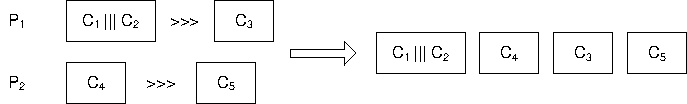
\includegraphics[scale=0.9]{multi.pdf} \\
%\captionof{figure}[Execution order of multithreaded programs]{Execution order of multithreaded programs}
%\end{center}

Assume we have two threads, $p_1$ and $p_2$. Command $c_1$ and $c_2$ forms a branch computation with combinator
($|||$). The whole branch computation is protected in a \co{protect} block and is executed atomically.
The atomic commands of $p_1$ and $p_2$ are executed alternatively as depicted in the figure.
No matter how the inputs are changed, the execution order of commands of $p_1$ and $p_2$ are still the same.
Since the execution time of branch computations is invisible to other threads, no {\em internal-timing}
channels can be exploited.

\section{The Run-time System}
\label{chap7:runtime}
% ArrowRef
% operational semantics?

This section explains the run-time system of FlowHaskellRef
and shows how the system prevents {\em internal-timing} channels.

\subsection{The Run-time Environment}
The run-time Environment in FlowHaskellRef is implemented by data type \co{FlowEnv} 
as following(in FlowArrowRef.hs):
\begin{Verbatim}[fontsize=\small]
data FlowEnv a = FlowEnv {
      user_data  :: a,                    
      ident      :: ThreadId        
      thread_que :: TVar [ThreadId],      
      p_count    :: Int,                   
   }
\end{Verbatim}
Field \co{user\_data} stores the data used as inputs and outputs of computations. 
Field \co{ident} stores the thread identity of current thread. 
Field \co{thread\_que} is a \co{TVar} pointed to a list of thread identities, while
field \co{p\_count} denotes how many nested \co{protect} blocks a current thread is inside.
The purposes of last two fields are explained in the following paragraphs.

\paragraph{Internal Thread Queue}
The behavior of schedulers in Haskell run-time system may differ from implementations to implementations. 
If the security of a program depends on certain property of a scheduler, a slightly change in the
scheduler may make a program regarded as secure before fail to obey information-flow policies.
Thus, a scheduler-independent run-time system is vital if we do not expect a scheduler to have certain property.
The thread queue is a global data
and can be accessed by all running threads in FlowHaskellRef. 
Only the thread whose identity is the same as the first element of the queue
can execute commands and the first element is put to the end of the queue after executing an atomic command.
In other words, the thread queue guarantees a round-robin execution order of all threads whatever
the scheduler of Haskell run-time system is, and thus is scheduler independent.

\paragraph{Nested Atomic Execution}
In the lock-based framework described in Sec.~\ref{chap7:atomicexecution}, the whole if-then-else statement
is in a \co{protect} block and thus only enclosed by a pair of \co{lock} and \co{unlock}. 
But in FlowHaskellRef, every single command is enclosed by a pair of \co{lock} 
and \co{unlock}. To achieve the effect as in the \co{protect} block, field \co{p\_count} in \co{FlowEnv}
is used to track if commands are in a \co{protect} block. Field \co{p\_count} is an integer that records
the number of nested \co{protect} blocks a command is inside.

\subsection{ArrowRef}
%ArrowRef
The run-time system of FlowHaskellRef is implemented in data type \co{ArrowRef}(in FlowArrowRef.hs). 
\begin{Verbatim}[fontsize=\small]
data ArrowRef a b = AR ((FlowEnv a) -> IO (FlowEnv b))
\end{Verbatim}
It is a function that takes a run-time environment (\co{FlowEnv} \co{a}) and returns a run-time environment
(\co{FlowEnv} \co{b}) in the IO monad. Data type \co{ArrowRef} is an {\em arrow} and has instances in
type class \co{Arrow} and \co{ArrowChoice}.

\subsection{Semantics for Commands}

\begin{figure}[t]
\[ \begin{array}{c}
   \inference[]{}{\config{\cod{arr}}{m}~->~\config{\cod{stop}}{m}} \quad
   \inference[]{\config{c_1}{m}~->~\config{\cod{stop}}{m'}}{\config{c_1;c_2}{m}~->~\config{c_2}{m'}} \\ \\
   \inference[]{id==(\cod{head}~q) \quad p==0}{\config{\cod{lockA}}{(id,q,p)}~->~\config{\cod{stop}}{(id,q,p)}} \quad
   \inference[]{id\not=(\cod{head}~q) \quad p==0}{\config{\cod{lockA}}{(id,q,p)}~->~\config{\cod{sleep}}{(id,q,p)}} \\ \\
   \inference[]{p > 0}{\config{\cod{lockA}}{(id,q,p)}~->~\config{\cod{stop}}{(id,q,p)}} \quad
   \inference[]{p==0}{\config{\cod{unlockA}}{(id,q,p)}~->~\config{\cod{stop}}{(id,\gamma(q),p)}} \\ \\
   \inference[]{p > 0}{\config{\cod{unlockA}}{(id,q,p)}~->~\config{\cod{stop}}{(id,q,p)}} \quad
   \inference[]{\config{\cod{lockA}}{m}~->~\config{\cod{stop}}{(id,q,p)}}
               {\config{\cod{hideA}}{m}~->~\config{\cod{stop}}{(id,q,p+1)}} \\ \\
   \inference[]{\config{\cod{unlockA}}{(id,q,p-1)}~->~\config{\cod{stop}}{m}}
               {\config{\cod{unhideA}}{(id,q,p)}~->~\config{\cod{stop}}{m}} \quad 
   \gamma(q)~=~(\cod{tail}~q)+\negthickspace +[(\cod{head}~q)]
   \end{array}
\]
\caption{Semantics for \co{ArrowRef} Commands}
\label{fig:semantics:arrowref}
\end{figure}

% Transactional lock and unlock avoid wait list problem and fairness is preserved by the thread queue.
In the lock-based framework, four new primitives in \co{ArrowRef} are developed. They are \co{lockA},
\co{unlockA}, \co{hideA}, and \co{unhideA}. The small-step semantics of these primitives are depicted 
in Figure~\ref{fig:semantics:arrowref}.
The command syntax is defined as following.
\begin{align*}
\cod{c}::=&~\cod{stop}~|~\cod{sleep}~|~\cod{arr}~|~c;c~|~\cod{lockA} \\
          &|~\cod{unlockA}~|~\cod{hideA}~|~\cod{unhideA}
\label{chap7:commandsyntax}
\end{align*}
A command finishes normally becomes \co{stop}.
Command \co{sleep} puts the current thread to sleep, and command \co{arr} represents any {\em arrows}
computation of \co{ArrowRef}. An environment \co{m}
is a three-tuple (\co{id},\co{q},\co{p}), which correspond to \co{ident}, \co{thread\_que},
\co{p\_count} in \co{FlowEnv}. A command \co{c} and an environment \co{m} form a 
{\em command configuration}, $\config{\cod{c}}{\cod{m}}$. Function \co{head} and $\gamma$ are
Haskell functions. Effects of command \co{arr}s in the memory are skipped here.

To avoid the wait list problem mentioned in Sec.~\ref{chap7:atomicexecution}, the implementation of
\co{lockA} and \co{unlockA} are based on STM Haskell~\cite{Harris:Marlow:Jones:Herlihy:PPoPP05}. 
The fairness, the reason that a wait list presents, is preserved by the internal thread queue.
Primitive \co{lockA} is implemented by an IO command \co{lock} as following(in FlowArrowRef.hs):
\begin{Verbatim}[fontsize=\small]
lock :: FlowEnv a -> IO Bool
lock env = if (p_count env) > 0
             then return False
             else atomically $
                  do que <- readTVar (thread_que env)
                     if head que /= (ident env)
                       then retry
                       else return True

lockA :: ArrowRef a a
lockA = AR (\env -> do lock env
                       return env)
\end{Verbatim}
Command \co{lock} first checks field \co{p\_count} to see if the current thread is in a \co{protect} block.
If yes, it will not try to get the lock again so it returns and execute commands.
Otherwise, the thread queue is read from the \co{TVar} \co{thread\_que} of the environment and checked if 
current thread is next thread which can execute commands. If it is not, a \co{retry} command is called
and the current thread is put to sleep until other threads modify the thread queue. If it is, \co{lock}
returns and the thread may executes commands that follows. Primitive \co{unlockA} is implemented by a
command \co{unlock} similar to \co{lock}.

The following shows how every single command is locked and unlocked using \co{lockA} and \co{unlockA}
(in FlowArrowRef.hs):
\begin{Verbatim}[fontsize=\small]
pure :: (b -> c) -> ArrowRef b c
pure f = lockA >>>
         AR (\env -> do b <- return $ f (user_data env)
                        return env{ user_data = b } )
         >>> unlockA
\end{Verbatim}
Every Haskell function lifted by combinator \co{pure} is regarded as one command.

The semantics of \co{protect} is implemented by a pair of \co{hideA} and \co{unhideA}.
Primitive \co{protect} is required for every branch command with high guard. In a lattice,
except label $\bot$, other labels can be high guard w.r.t. some other labels. Therefore,
an approximation is made to protect all branch computations. In FlowHaskellRef, combinator
(\arrowop{+}) and ($|||$) create branch computations and the computations are enclosed by \co{hideA} and 
\co{unhideA}. The following is the implementation of field \co{computation} of (\arrowop{+})
(in FlowArrowRef.hs):
\begin{Verbatim}[fontsize=\small]
computation = (\upd -> hideA >>> 
                       (c1 (upd.(replaceSecType sub1)) 
                        +++ 
                        c2 (upd.(replaceSecType sub2))) 
                       >>> unhideA)
\end{Verbatim}

Primitives of locks and hides have to be pairwise. It is the responsibility of the library developers to
maintain such invariant when creating new primitives in FlowHaskellRef.

\section{New Combinators of FlowHaskellRef}
% forkRef, atomicA, iterateA(maybe in chap4)
\begin{figure}[t]
\[ \begin{array}{c}
   \inference[$FORK$]{pc,\Delta,\Theta \proves f~:~\res{\typn{1}}{\sts{1}}~->~\res{\typn{2}}{\sts{2}}} 
                     {pc,\Delta,\Theta \proves \cod{forkRef}~f~:~\res{\typn{1}}{\sts{1}}~->~\res{()}{\bot}}  \\ \\
   \inference[$ATOMIC$]{pc,\Delta,\Theta \proves f~:~\res{\typn{1}}{\sts{1}}~->~\res{\typn{2}}{\sts{2}}}
                       {pc,\Delta,\Theta \proves \cod{atomicA}~f~:~\res{\typn{1}}{\sts{1}}~->~\res{\typn{2}}{\sts{2}}} \\
   \end{array}
\]
\caption{Type system of \co{forkRef} and \co{atomicA}}
\label{fig:fork:typesystem}
\end{figure}

Two new combinators are introduced in FlowHaskellRef. Combinator \co{forkRef} supports dynamic thread
creation, while combinator \co{atomicA} provides atomic execution of a sequence of commands. The type
system of the two combinators are as in Figure~\ref{fig:fork:typesystem}.

Combinator \co{forkRef} directs the input to the computation of the \co{FlowArrowRef} passed to \co{forkRef}.
A new thread is created with an exception handler. If exception \co{undefined}
is raised in one of the running thread, all threads are killed immediately. Thus, no information
is leaked. The output security type of \co{forkRef} is $\bot$ because only a unit is returned
whatever the input is.

Combinator \co{atomicA} encloses a \co{FlowArrowRef} computation with a
\co{hideA} and \co{unhideA} pair. The whole computation is regarded as a single command and runs atomically.

\chapter{Case Study of Multithreaded FlowHaskellRef}
Two examples are implemented in FlowHaskellRef to demonstrate {\em internal-timing} channels
are eliminated. The first example is a small experiment to evaluate the correctness and efficiency
of the run-time system. The second case study is an on-line shopping simulation. An attack program is provided
to show that FlowHaskellRef guarantees multithreaded information-flow policies.

\section{Experimental Example}
\label{chap8:expexample}
In this example, a multithreaded program that exhibits {\em internal-timing} channels is implemented
as follows(in MultiExp.hs):
\begin{Verbatim}[fontsize=\small]
t1 :: Int -> Int -> FlowArrowRef TriLabel ArrowRef () Int
t1 v dtime = 
   lowerA LOW (pure (\() -> 99)) >>>
   createRef LOW >>>
   (idRef &&& forkRef t2) >>>
   (second
     (pure (\() -> v) >>>
      pure (\i -> if i > 5 then Left dtime else Right 0) >>>
      ((skipRef >>> tagRef HIGH)
       |||
       (skipRef >>> tagRef HIGH)
      )
     )) >>>
   second (lowerA LOW (pure (\_ -> 1))) >>> 
   (fstPair &&& (writeRef >>> pure (\() -> 10000) >>> skipRef ))
   >>> fstPair >>>
   readRef (SecLabel (Lab LOW))

t2 :: FlowArrowRef TriLabel ArrowRef (SecRef TriLabel Int) ()
t2 = ( idRef &&& lowerA LOW (pure (\_ -> 2))) >>> writeRef
\end{Verbatim}
Thread \co{t1} creates a \co{LOW} reference and then dynamically creates a new thread \co{t2}.
Thread \co{t2} writes integer 2 to the reference and finishes.
Depending on \co{HIGH} value \co{v}, thread \co{t1} has different executing steps in each branch.
Primitive \co{skipRef} takes an integer \co{k} as the input and performs \co{k} empty steps.
Each empty step is a \co{return} statement in the IO monad.
In the example, if $\cod{v}>5$, then the branch executes \co{dtime} empty steps. Otherwise, zero
empty step is executed. Then, thread \co{t1} writes integer 1 to the reference. After executing 10000
empty steps, the content of the reference is read out as the output.

The same program is run in two run-time systems: \co{R1} and \co{R2}.
Run-time system \co{R1} is the one adopted in FlowHaskellRef.
Run-time system \co{R2} is similar to \co{R1} but without using \co{lockA} and \co{unlockA} to execute each
command atomically and also \co{hideA} and \co{unhideA} to protect a branch computation.
For each test case, the program is run 100 times. 
The results with \co{dtime} = 10000 are listed in Table~\ref{table:r1:10000} and Table~\ref{table:r2:10000},
while the results with \co{dtime} = 15000 are shown in Table~\ref{table:r1:15000} and Table~\ref{table:r2:15000}.
If \co{v} = 10, the branch that runs \co{dtime} empty steps is chosen. Otherwise, the branch that
runs zero empty step is chosen. Column {\bf Output} records the frequency of the outputs, 1 or 2, among
100 runs. The running time of a test case is recorded in column {\bf Time}.
\footnote{The program is run on a laptop with Pentium M 1.5 GHz and 512 MB RAM.}

When the program runs in the run-time system \co{R1}, the output is always 1 no matter which branch computation 
is chosen. But when the program runs in the run-time system \co{R2}, the statistic results in 
Table~\ref{table:r2:10000} and Table~\ref{table:r2:15000} shows the {\em internal-timing} channels.
If \co{v} = 10, the probability of 1 as the output
is higher because the statement that assign 1 to the reference in \co{t1} tends to execute 
later than the statement that assign 2 to the reference in \co{t2}. On the other hand, if 
\co{v} = 0, the execution order of the two assignments tends to be reversed. Thus, the probability of 2
as the output is higher. This assumption is corroborated by comparing the results in Table~\ref{table:r2:10000}
and Table~\ref{table:r2:15000}. When \co{v} = 10, the larger \co{dtime} is the higher probability
of 1 as the output becomes.

The running time of the program in run-time system \co{R1} are about three times slower than that in
run-time system \co{R2}. The huge overhead is introduced by the internal thread queue. Most of the threads
that are scheduled by the scheduler are put to sleep again because they are not the next thread which 
can execute commands. However, the cost is normally tolerable since only small part of a program that involves
secret data is built in FlowHaskellRef. The remaining part of the program keeps the same efficiency as
before.

\begin{table}[t]
\centering
\begin{tabular}{|ccc||ccc|}
\hline
{\bf Value of} \co{v}& {\bf Output} (1,2)& {\bf Time}({\bf Sec.}) & 
{\bf Value of} \co{v}& {\bf Output} (1,2)& {\bf Time}({\bf Sec.})\\ \hline
10 & (100,0) & 43  & 0 & (100,0) & 34 \\
10 & (100,0) & 44  & 0 & (100,0) & 34 \\
10 & (100,0) & 43  & 0 & (100,0) & 34 \\
10 & (100,0) & 44  & 0 & (100,0) & 34 \\
10 & (100,0) & 43  & 0 & (100,0) & 34 \\
\hline
\end{tabular}
\caption{Result in \co{R1} with $\cod{dtime} = 10000$}
\label{table:r1:10000}
\end{table}

\begin{table}[t]
\centering
\begin{tabular}{|ccc||ccc|}
\hline
{\bf Value of} \co{v}& {\bf Output} (1,2)& {\bf Time}({\bf Sec.}) & 
{\bf Value of} \co{v}& {\bf Output} (1,2)& {\bf Time}({\bf Sec.})\\ \hline
10 & (83,17) & 16  & 0 & (15,85) & 12 \\
10 & (90,10) & 15  & 0 & (13,87) & 12 \\
10 & (86,14) & 16  & 0 & (16,84) & 12 \\
10 & (90,10) & 16  & 0 & (18,82) & 13 \\
10 & (89,11) & 16  & 0 & (11,89) & 13 \\
\hline
\end{tabular}
\caption{Result in \co{R2} with $\cod{dtime} = 10000$}
\label{table:r2:10000}
\end{table}

\begin{table}[t]
\centering
\begin{tabular}{|ccc||ccc|}
\hline
{\bf Value of} \co{v}& {\bf Output} (1,2)& {\bf Time}({\bf Sec.}) & 
{\bf Value of} \co{v}& {\bf Output} (1,2)& {\bf Time}({\bf Sec.})\\ \hline
10 & (100,0) & 47  & 0 & (100,0) & 35 \\
10 & (100,0) & 48  & 0 & (100,0) & 35 \\
10 & (100,0) & 47  & 0 & (100,0) & 35 \\
10 & (100,0) & 47  & 0 & (100,0) & 33 \\
10 & (100,0) & 47  & 0 & (100,0) & 35 \\
\hline
\end{tabular}
\caption{Result in \co{R1} with $\cod{dtime} = 15000$}
\label{table:r1:15000}
\end{table}

\begin{table}[t]
\centering
\begin{tabular}{|ccc||ccc|}
\hline
{\bf Value of} \co{v}& {\bf Output} (1,2)& {\bf Time}({\bf Sec.}) & 
{\bf Value of} \co{v}& {\bf Output} (1,2)& {\bf Time}({\bf Sec.})\\ \hline
10 & (96,4) & 18  & 0 & (18,82) & 12 \\
10 & (98,2) & 18  & 0 & (17,83) & 12 \\
10 & (98,2) & 17  & 0 & (20,80) & 12 \\
10 & (93,7) & 18  & 0 & (12,88) & 12 \\
10 & (95,5) & 17  & 0 & (19,81) & 12 \\
\hline
\end{tabular}
\caption{Result in \co{R2} with $\cod{dtime} = 15000$}
\label{table:r2:15000}
\end{table}

\section{On-line Shopping Simulation}
\label{chap8:shopping}
% scenario (simulation)
% attack program (statistic attack to guess credit card)
In this case study, a program that simulates an on-line shopping application is implemented in FlowHaskellRef.
The program is run in two run-time systems, called \co{R1} and \co{R2}. Run-time system \co{R1} is 
as described in Sec.~\ref{chap7:runtime}, while run-time system \co{R2} does not use \co{lockA}, \co{unlockA},
\co{hideA}, and \co{unhideA} to protect branch computations. An attack program trying to exploit
{\em internal-timing} channels is developed to evaluate different run-time systems.

\subsection{Simulation Program}
To purchase a product, each client sends a name, a telephone number, a credit card number, and an address to
a service program provided by the company that sells the product. The service program is divided into
three phases. The first phase is implemented by a trusted procedure to protect each data with proper
security types. The name, the telephone number, and the address are public data and protected by label \co{LOW}. 
The credit card number is regarded as a secret data and thus protected by label \co{HIGH}. 
In the second phase, these protected data are processed by a procedure, call \co{serverProcess},
which is not trusted. The type signature of the function is as following(in Shopping.hs):
\begin{Verbatim}[fontsize=\small]
type Protected b c = FlowArrowRef TriLabel ArrowRef b c

serverProcess :: Protected ((SRef TriLabel [CNum], 
                             SRef TriLabel [PubItem]),
                            (CNum,((Name,Tel),Addr)))
                           ()
\end{Verbatim}
Function \co{serverProcess} take two references and a client's information. The first reference stores
credit card number and the content is protected by security type (\co{SecLabel} (\co{Lab} \co{HIGH})). 
The second reference stores other public information and thus protected by
(\co{SecLabel} (\co{Lab} \co{LOW})).
In the simulation, the process of data is simply to separate secret data and public data, 
and store them in the corresponding references.
The third phase is to process the public and the secret references by a trusted procedure.
In the simulation, the public data are printed on the screen.

A malicious program can be implemented in \co{serverProcess} and try to leak information about the credit card 
number to the public reference. Those information can be collected after the public data are printed in the 
third phase. 

\subsection{Malicious Program}
The malicious program exploits the {\em internal timing} channels to infer a credit card number and store it
in the public reference. Similar techniques as in Sec.~\ref{chap8:expexample} is adopted. 
An attack reference, which is public, is created and its final value depends on a secret data.
See Sec.~\ref{chap8:expexample} for details.
However, the attack only reveals one bit information each time. In the malicious program, the attack
is magnified by repeating itself several times to infer all bits of a credit card number. 
The attack begin with the most significant bit of a credit card number. Assume the credit card number has
\co{n} bits. The following code shows how to infer this bit(in Shopping.hs).
\begin{Verbatim}[fontsize=\small]
lowerA HIGH (pure (\(k,cnum) -> if cnum >= 2^k 
                                  then Left 30000 
                                  else Right 0)) >>>
                   ((skipRef >>> tagRef HIGH)
                    |||
                    (skipRef >>> tagRef HIGH))
\end{Verbatim}
Variable $\cod{k} =\cod{n} -1$ in this case. If the credit card number, \co{cnum}, is larger than or equal to $2^{n-1}$, 
the branch taking $30000$ empty steps is chosen. Otherwise, the branch taking $0$ empty steps is run.  
Based on the final value of the attack reference, the information of this 
bit is exploited and appended to the public address field. 
If $\cod{cnum} >=2^{n-1}$, $\cod{cnum} -2^{n-1}$ becomes the new \co{cnum}. The whole procedure
is repeated to infer next bit with $\cod{k} =\cod{n} -2$.
By performing the attack \co{n} times, every bit of the credit card number is revealed in the address field and 
is written to the public reference later.

We assume a credit card number has 16 digits in decimal and thus at most 53 bits. 
The client information is as following:
\begin{Verbatim}[fontsize=\small]
Name  : Bob
Tel.  : 07042312323
CNum. : 9999999999999999
Addr. : Rotary 2K-1234, Gothenburg.
\end{Verbatim}
The binary representation of the credit card number is:
\begin{Verbatim}[fontsize=\small]
100011100001101111001001101111110000001111111111111111
\end{Verbatim}
The malicious program is run in both run-time system \co{R1} and \co{R2}. 

\subsubsection{Run-time system \co{R1}}
When the malicious program executes in run-time system \co{R1}, the output is as following every
time it runs.
\begin{Verbatim}[fontsize=\small]
### Client ###
Name : Bob
Tel  : 07042312323
Addr : Rotary 2K-1234, Gothenburg.
000000000000000000000000000000000000000000000000000000
\end{Verbatim}
The last line shows the bits inferred from the credit card number. They are all zeros so no information of
the credit card number is revealed.

\subsubsection{Run-time system \co{R2}}

\begin{table}[t]
\centering
\begin{tabular}{lcc}
{\bf Run No}. & {\bf Result} & {\bf Time}({\bf Sec}.) \\ \hline \\
1  & 101011111001111111111011101111110000011111111111111111 & 27 \\
2  & 110011100001101111011101101111010000001111111111111111 & 27 \\
3  & 101011100001101111101001101111110000001111111111111111 & 28 \\ 
4  & 100011100101101111001001101111110000001111111111111011 & 28 \\
5  & 100011100001101111001001101111110100001111111111111111 & 29 \\
6  & 100011100001101111001000101111110001011111111111111111 & 29 \\
7  & 100011100001101111011001111111110000001111111111111111 & 28 \\
8  & 100111100001101111001101101111110000001111111111111111 & 28 \\
9  & 100010100001101111001001101111110000001111111111111111 & 27 \\
10 & 101011100001111111001001101111110000001111111111111111 & 28 \\
\\ \hline \\
sum   & 0979010999*008000087089109000010*9*9*80000000000000100 &    \\
\\ \hline \\
cnum' & 100011100001101111001001101111110000001111111111111111 & \\
\end{tabular}
\caption{Statistical results of the malicious program}
\label{table:chap8:shopping}
\end{table}

When the malicious program runs in run-time system \co{R2}, one of the output is as following.
\begin{Verbatim}[fontsize=\small]
### Client ###
Name : Bob
Tel  : 07042312323
Addr : Rotary 2K-1234, Gothenburg.
101011111001111111111011101111110000011111111111111111
\end{Verbatim}
There are usually 2 or 3 bits that are not correctly inferred. This is probably because the execution time of 
empty steps is slightly different in each run. Besides, we do not know how the scheduler of the Haskell run-time
system treats a fork command.
However, if the attack is repeated several times, we can still infer the credit card number with high
confidence. Table~\ref{table:chap8:shopping} lists the results and the corresponding running times in ten runs. 
The row \co{sum} records how many times 0 appears in a certain digit. Symbol * means ten times.
For instance, the second digit of row \co{sum} is 9. This means that 0 appears in the second digit
of the result nine times among the ten runs. The inferred credit card number, \co{cnum'}, is decided by row \co{sum}.
If the frequency of 0 appearing in a digit is higher than five times, the digit is inferred as 0.
Otherwise, the digit is inferred as 1. Row \co{cnum'} is the final credit card number inferred, which
is the same as the real credit card number. By this method, an attacker can obtain the credit card number of a client
within five minutes.\footnote{The program is run on a laptop with Pentium M 1.5 GHz and 512 MB RAM.}




\chapter{Discussions and Conclusions}

\section{Combinator \co{lowerA}}
% summary the function of lowerA
% why not deduce output security types in pure?
% lowerA provides more flexibility than pure which is important(input filtering)
% -- more constraints are required.
Combinator \co{lowerA} is created for transforming combinator \co{pure}.
The inputs of \co{lowerA} first pass through an input filtering function, and
the output security types are deduced from the output types.
The reason that those mechanisms are not implemented in combinator \co{pure}
is because every type used has to implement overloading functions in some Haskell type classes.
To be generic, some type constraints are required in the type signature of
\co{pure}. For instance, to deduce output security types, the {\em arrow} should be
an instance of type class \co{DowngradeArrow}. The type signature of \co{pure}
is expected as following:
\begin{Verbatim}[fontsize=\small]
pure :: DowngradArrow SecType l a b c => 
        (b -> c) -> a b c
\end{Verbatim}
However, the type signature of \co{pure} is fixed and cannot be changed.

With the input filtering function, combinator \co{lowerA} provides more flexibility than
the \co{pure} in the previous work. Combinator \co{lowerA} may takes secret inputs and produces
public outputs as long as the outputs do not depend on secret inputs. This has been proved
useful in the case studies. At some point of a program, the programmers may like to discard all
secret data and begin with a data of lower security level. 
For example, in the bank simulation cast study, computation
\co{atm\_nonce} takes a unit with security level \co{ATM\_BANK} and returns a nonce. 
We may like to get the nonce after processing some data of security level \co{BANK}.
Consider the following program.
\begin{Verbatim}[fontsize=\small]
lowerA BANK (pure (\x -> x)) >>>
lowerA ATM_BANK (pure (\i -> ())) >>> atm_nonce
\end{Verbatim}
The inputs \co{i} with security level \co{BANK} is discarded and a unit with security level 
\co{ATM\_BANK} is returned in the \co{lowerA}. Without this flexibility, the programmers have to
declassify the unit. Nevertheless, more declassification require more manual inspections.

However, the cost of the flexibility is that part of checking is postponed to the execution time of
underlying computations. Value \co{undefined} causes an exception and aborts a running computation
when it is used. To prevent such delayed checking, the programmers may use combinator \co{equalA} instead.
Combinator \co{equalA} has a strict constraint on the input security types but guarantees all constraints
are checked when certifying a FlowHaskellRef program.

\section{Run-time Checking of References}
The security types for a reference's content is invariant in the sub-typing relation because 
it can be shared by different references.
When a reference pass through \co{lowerA}, it relies on the read projection function and
write protection function to guarantee the invariant.
However, this delays the constraint checking of references to the second phase when the
desired computation is running.
Because an illegal read becomes undefined and an illegal write raise an error exception,
the running program is stopped immediately before any secret information is leaked.
But, still, one disadvantage of this approach is that debugging becomes difficult. 
For applications that program abortion during service is intolerable, 
every branch of the programs has to be tested once before running for service. 
This makes testing a program more complex.

\section{Closing Timing Channels via Internal Scheduler}
% timing channel is produced by the program and the scheduler
% static type system for programs are usually too restrictive
% to accept more program, more assumption on the scheduler
% have more expressiveness : 1. interact with scheduler
% simple solution : an internal scheduler
% pros : easy to implement, scheduler independent
% cons : overhead is huge(but only small part is written in the sub-language)
% future work : ??? 
In multithreaded programs, it is the interleaving of the threads that opens the timing channels. 
However, the interleaving of the threads is affected not only by the programs but also by the schedulers.
Different schedulers may create timing channels in different ways.

There has been some studies showing how to apply static type system techniques to reject insecure
programs~\cite{Castellani:Boudol:TCS02,Volpano:Smith:Probabilistic,Zdancewic:Myers:CSFW03}. 
One of the advantages of static type system is the programs have no run-time overhead.
But those type systems are normally too restrictive or require non-standard semantics. 
Some of them may reject intuitively secure and useful programs and are not practical for
real-world applications.
Others retain the permissiveness to accept more secure programs but make assumptions about schedulers. 
Many of the assumptions are hard to achieve in practice. For instance, a non-deterministic scheduler.
However, an observation is that more regulation in schedulers provides higher permissiveness to accept secure
programs.

FlowHaskellRef chooses to implement an internal scheduler to eliminate internal timing channels.
This approach accepts all original programs accepted in the sequential version of FlowHaskellRef. The programmers
write programs as before without worrying what kind of pattern may create timing channels.
Besides, the approach is scheduler independent. Programs written in FlowHaskellRef preserve
information-flow policies in all Haskell run-time system.
Moreover, the implementation is simple and has potentially fewer bugs.
However, the cost of the approach with high permissiveness is a non-trivial overhead. 
FlowArrowRef implements the internal scheduler by a thread queue in a round-robin fashion. 
Threads are scheduled by two schedulers. When scheduled by Haskell run-time system, if
the thread is not scheduled by the internal thread queue, it is put to sleep. 
In worst case, every thread is scheduled once by Haskell run-time system and put to sleep before the thread
scheduled by the internal scheduler is scheduled.

However, FlowHaskellRef, as an embedded language, can be used along with normal Haskell to build programs.
In many cases, only small part of a system that involves secret information is 
written in FlowHaskellRef. Other part of the system can still be written in normal Haskell. 
The efficiency cost is comparatively low in exchange for no information leak.

To reduce the overhead, one way would be to give up the internal scheduler and have interactions with the scheduler 
of Haskell run-time system. Similar approach has been explored by Russo and Sabelfeld~\cite{Russo:Sabelfeld:CSFW06}.

\section{Future Work}
\subsection{Decentralized Label Model}
As described in Sec.~\ref{chap6:eval:flowhaskellref}, dummy labels are required for the integrity
of the lattice in the case study. This is because a lattice has a global top element that
represents a universally trusted authority. However, such authority in real-world situations are normally 
not existed. There are usually authorities that do not trust each other but cooperate to complete
interesting tasks. Decentralized label model(DLM)~\cite{Myers:Liskov:TSEM2000} has been shown suitable for
modelling these situations.

\subsection{Arrow Syntax Transformation}
Paterson~\cite{Paterson:ICFP01} proposes a \co{do}-notation like syntax transformation
for {\em arrows}. It allows the programmers to write pointed {\em arrow} code. 
Pointed programming style is favored by some people because it provides a similar
reasoning style as in imperative languages.
The transformation relies heavily on combinator \co{pure} to organize the structures of data. 
However, to build useful programs in FlowHaskellRef, combinator \co{pure} is normally used in 
conjunction with combinator \co{lowerA} to deduce output security types. Thus, the syntax transformation 
cannot be used for FlowHaskellRef. 

New syntax transformation for FlowHaskellRef can be extended easily based on current syntax transformation.
The only difference is that all \co{pure} combinators generated in the transformation are wrapped by a \co{lowerA} 
combinator. The programmers, nevertheless, still need to provide a security label as before for \co{lowerA}.

\subsection{Multiple Authorities in a Secure Program}
In FlowHaskellRef, only one authority can be used to certify a secure program. This is sufficient for
sequential programs. Assume a program requires cooperation of two different authorities, 
called \co{A} and \co{B}. It can be written in several small programs that only require one of the authority.
If a sub-program which belongs to authority \co{B} requires data from the other sub-program which belongs to
authority \co{A}, the second program is certified by authority \co{A} and then pass the output to the
first program. 

The situation is different for multithreaded programs in FlowHaskellRef. To guarantee no {\em internal-timing}
channels in a multithreaded program, all dynamic threads have to be created via the primitives in 
FlowHaskellRef. This means the whole secure program only belongs to one authority. Consider an auction simulation
program in the following figure. 

%\begin{center}
%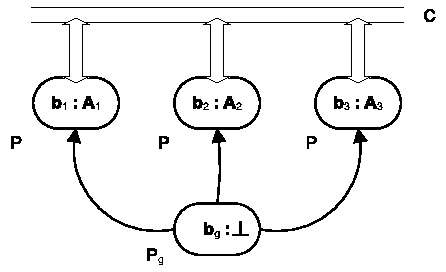
\includegraphics[scale=0.9]{bidder.pdf} \\
%\captionof{figure}[Auction simulation]{Auction simulation}
%\end{center}

There is a public global bid, $b_g$, which can be accessed by bidders. 
The global bid is maintained by program $P_g$. It create a client thread, $P$, for each 
bidder that has his own private bid, $b_i$.
The snapshot is after three bidders joined the auction. 
There is a public channel, $C$, for bidders to exchange messages that are not related to their private bids.
To protect program $P$ from leaking the private bid $p_i$ in the public channel, each client's bid is protected
by a different security level, $A_i$.  
The auction proceeds with each client compares its bid $b_i$ with the global bit $b_g$.
If $b_i>b_g$, the client increases $b_g$ by 1. Otherwise, the client loses and leaves the auction.
The increment of $b_g$ depends on private bid so declassification is required.
Thus, client thread with bid $b_i$ should be certified at least with authority $A_i$.
However, the program cannot be implemented in FlowHaskellRef because only one authority can be used in
the program. To allow all legal declassification, an authority higher than all $A_i$s are required.
But this allows clients to read other bidders' bids on the public channel.
Mechanisms to compose programs of different authorities are necessary to build the auction simulation program.


\section{Conclusion}
% Function : sequential information flow, references, precise security types, 
%            less burden of programmers(unification), close internal timing channel,
%            case study
% Advantage : low cost to migrate, practical, light-weighted, scheduler independent, 
%             full permisiveness as before.
% Cons : reference checking is delayed to run-time, debug message is not clear
FlowHaskellRef extends FlowHaskell with reference manipulation and secure multithreaded programming.
The new contributions are listed as following:
\begin{enumerate}
\item Complex security types permits more accurate description of data
\item Reference manipulation provides possibility of shared resource
\item Unification mechanism infers security types automatically and mitigates the responsibility of the programmers
\item Scheduler-independent run-time system eliminates {\em internal-timing} channels in multithreaded programming
\item Two full case studies to evaluate FlowHaskellRef
\end{enumerate}

The design choices of FlowHaskellRef are mainly of practical concerns. 
It is aimed to provide the programmers with an easy-to-use and expressive secure language.
As a light-weighted tool, the migrating cost is much lower comparing to full-fledged security languages
like Jif~\cite{jif} and FlowCaml~\cite{FlowCaml}.
The programmers can write only security-related part of a program in FlowHaskellRef and switch between 
FlowHaskellRef and Haskell seamlessly.

On the other hand, FlowHaskellRef also have some limitations. First, the certification of a program is at
run-time. This makes the testing of a FlowHaskellRef program more difficult. A FlowHaskellRef program has to be 
run at least once to ensure all constraints are satisfied. Besides, the same checking is performed every time
the program runs. Second, the debugging message is not clear. All constraints are collected at run-time so
the information of where a constraint comes from is hard to provide.


\bibliographystyle{abbrv}
\bibliography{literature}



\end{document}
